% Scope-aware manuscript source prepared from the AutoFE-ShiftBench benchmark.
% Existing result files are referenced read-only; this source does not
% regenerate or modify them.
\documentclass[preprint,12pt]{elsarticle}

\usepackage[utf8]{inputenc}
\usepackage[T1]{fontenc}
\usepackage{lmodern}
\usepackage{microtype}
\usepackage{amsmath,amssymb}
\usepackage{booktabs}
\usepackage{graphicx}
\usepackage{xcolor}
\usepackage{array}
\usepackage{enumitem}
\usepackage{float}
\usepackage[hidelinks]{hyperref}

% Elsevier's correspondence macros are valid in the printed front matter but
% are not valid PDF-bookmark tokens.  Suppress only those tokens in metadata.
\makeatletter
\pdfstringdefDisableCommands{%
  \def\corref#1{}%
  \def\cortext#1{}%
  \def\ead#1{}%
  \def\cnotenum#1{}%
  \def\@corref#1{}%
}
\makeatother

\newcommand{\AUC}{\operatorname{AUC}}
\newcommand{\E}{\mathbb{E}}

\journal{Knowledge-Based Systems}
% The complete figure set is bundled inside paper/figures/ so this directory
% can be copied to a clean LaTeX environment without repository-relative paths.
\graphicspath{{figures/}}

\begin{document}

\begin{frontmatter}

\title{When More Features Hurt: Feature-Synthesis Variance Amplification in Automated Feature Engineering}

% Author and affiliation metadata supplied for this manuscript package.
\author[inst1]{Md. Shoaib Uddin Chanda\corref{cor1}}
\ead{mdshoaibuddinchanda@gmail.com}
\cortext[cor1]{Corresponding author.}
\author[inst1]{Mohammed Abdur Razzaq}
\ead{160925748170@lords.ac.in}
\author[inst1]{Mohammed Abdul Razzak}
\ead{abdulrazzak.m2008@gmail.com}
\author[inst2]{Ayesha Mahveen}
\ead{24321abb0b@brecw.ac.in}
\address[inst1]{Lords Institute of Engineering \& Technology}
\address[inst2]{Bhoj Reddy Engineering College for Women}

\begin{abstract}
Automated feature engineering (AutoFE) is intended to discover useful representations without hand-crafted domain rules, but the additional search space can also amplify noise, collinearity, and computational cost.  We hypothesize that generated arithmetic representations can amplify perturbations in the original feature space, increasing estimator variance, computational complexity, and the train--test generalization gap.  We call this mechanism Feature-Synthesis Variance Amplification (FSVA).  We evaluate AutoFE-ShiftBench, whose configured design contains 25 OpenML tabular data sets, five seeds, five folds, fourteen training-data conditions, seven pipelines, and ten classifiers.  The confirmatory analysis is restricted to the 22 data sets with substantial completed coverage: 538,972 evaluation records are available in this scope, while two large data sets were stopped during long-running final blocks and one configured data set has no completed primary records.  Across the primary scope, capped raw-feature baselines obtain mean ROC--AUC values of 0.8263 (Raw), 0.8263 (variance-ranked), and 0.8262 (mutual-information-ranked).  Addition/subtraction-only AutoFE is close at 0.8237, whereas mutual-information selection, randomized selection, and unrestricted baseline synthesis obtain 0.7985, 0.7804, and 0.7481, respectively.  The direction is consistent with larger train--test gaps and higher feature-generation cost for the less constrained AutoFE variants.  These results support a bounded conclusion: in this benchmark, unrestricted synthesis did not improve generalization under controlled corruption of the training data.  They do not establish that AutoFE is universally harmful.  We therefore separate completed evidence from stopped runs, quantify implementation threats to validity, and provide regenerated vector figures and a reproducible manuscript package.
\end{abstract}

\begin{keyword}
automated feature engineering \sep feature synthesis \sep distribution robustness \sep tabular classification \sep reproducibility \sep benchmarking
\end{keyword}

\end{frontmatter}

\section{Introduction}
\label{sec:introduction}

Feature construction is a central part of applied machine learning.  Classical feature selection work emphasizes that additional variables can increase variance and computational cost when they are weakly informative or redundant \citep{guyon2003}.  Automated machine learning systems and feature-synthesis libraries make this process accessible by searching transformations at scale \citep{feurer2015,olson2019,kanter2015}.  The same automation creates a practical question: when does a larger representation improve held-out performance, and when does it merely make the learner fit artifacts of the training sample?

The prevailing design proxy in automated feature engineering is feature quantity: a larger candidate library is often treated as a route to greater predictive power.  That proxy is incomplete because a feature is useful only if its signal survives sampling noise, perturbation, and deployment-like cost constraints.  What remains insufficiently tested is whether feature-space expansion improves robust generalization when the data, operator algebra, model family, and computational budget are controlled simultaneously.  Accordingly, this study evaluates AutoFE by the reliability of the retained features rather than by the number of generated features.

We use FSVA as a testable framework rather than as a label for an empirical ranking.  In its simplest form, a feature generator $g$ maps a perturbed input $x+\varepsilon$ to $g(x+\varepsilon)$; the Jacobian, product/ratio error propagation, effective degrees of freedom, and finite-search maximum quantify four routes by which synthesis can increase generalization risk.  The benchmark does not directly observe every latent quantity, so the resulting equations define falsifiable mechanisms and observable predictions rather than a universal theorem about AutoFE.

This paper studies that question using AutoFE-ShiftBench, a repeated tabular-classification benchmark with controlled perturbations applied to the training partition.  The protocol records predictive metrics, feature counts, resident-memory deltas, and phase timings for raw-feature and synthesized-feature pipelines.  Several very large evaluations were terminated after multi-hour linear-model tails; we therefore establish the inferential scope before drawing conclusions and distinguish completed evidence from computationally censored evaluations.

The contributions are fivefold:
\begin{enumerate}[leftmargin=*]
  \item We define a primary 22-dataset analysis scope and reconcile it with the configured 25-dataset grid and the 560,002 completed evaluation records.
  \item We compare three capped raw-feature baselines with four AutoFE variants across ten classifiers and fourteen training-data conditions.
  \item We formulate the Feature-Synthesis Variance Amplification (FSVA) effect as a mechanistic account linking operator sensitivity, redundancy, effective degrees of freedom, and search multiplicity to generalization risk, with equations and falsifiable predictions.
  \item We evaluate observable FSVA implications across the 538,972 completed primary-scope records, reporting performance, train--test gaps, robustness curves, feature dimensionality, computational cost, and a cost-normalized Feature Utility Ratio without treating stopped datasets as completed observations.
  \item We document validity boundaries, including training-only corruption, baseline collapse, non-reproducible perturbation seeds, incomplete multiclass metrics, and swallowed worker failures, so that the benchmark can be re-run or extended before confirmatory submission.
\end{enumerate}

\begin{figure}[H]
\centering
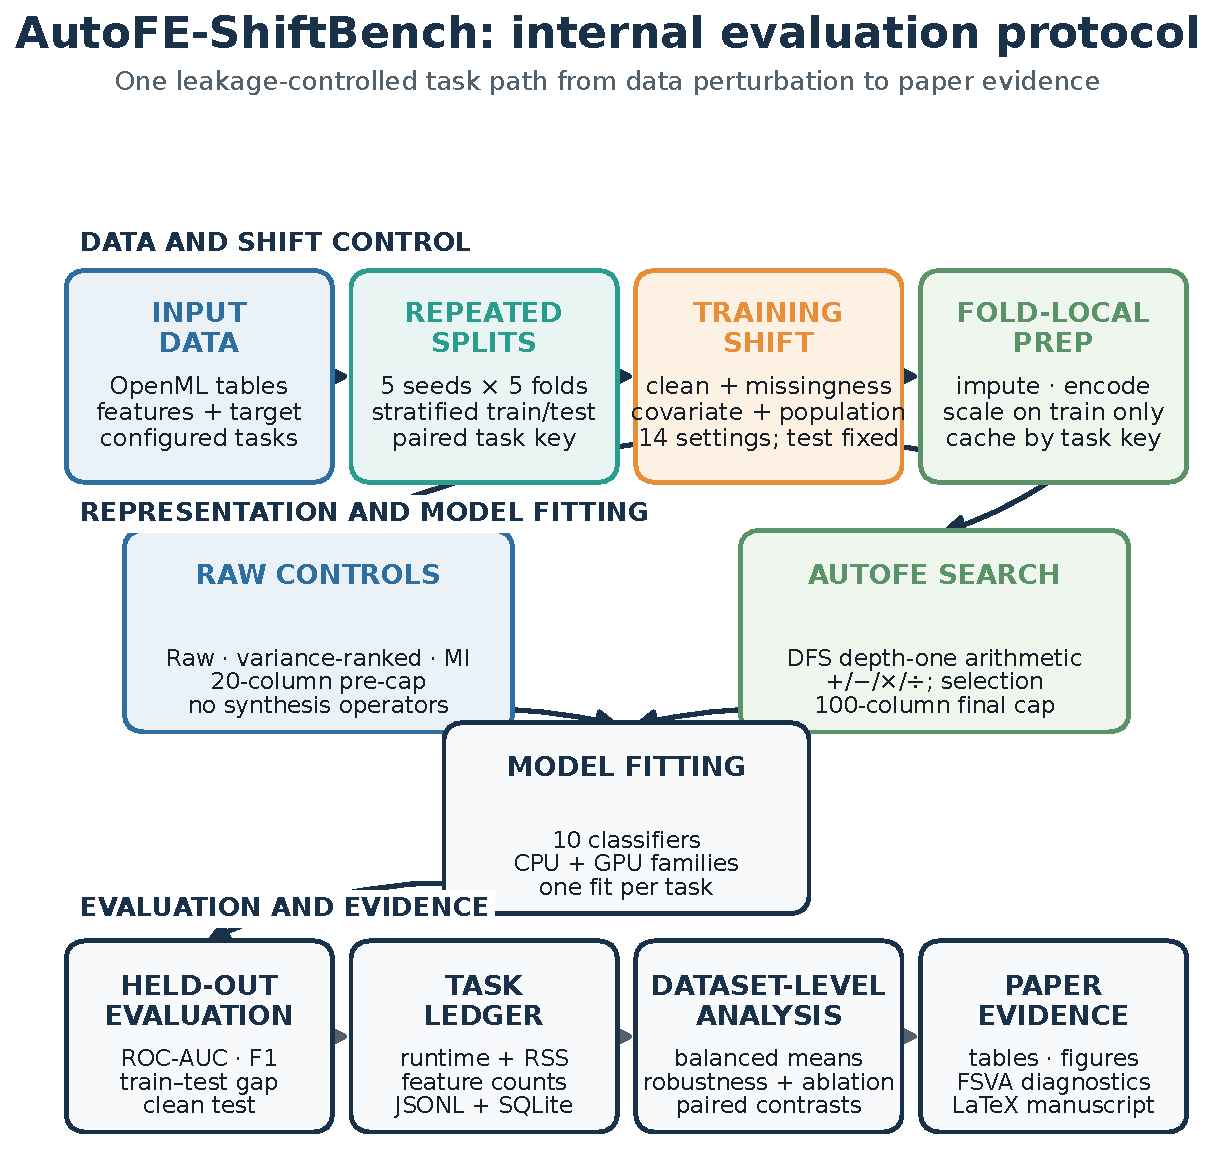
\includegraphics[width=\linewidth]{AutoFE_ShiftBench_Workflow.pdf}
\caption{Internal evaluation protocol.  Each task follows a leakage-controlled path from repeated train/test splitting and training-only perturbation through fold-local preprocessing, the capped raw-feature and AutoFE representation branches, model fitting, held-out evaluation, task-level logging, and data-set-level analysis.  Run-completion exceptions are reported in the Analysis scope and are not encoded in this method diagram.}
\label{fig:workflow}
\end{figure}

\subsection{Research gap and falsifiable questions}
\label{sec:questions}
The literature establishes that feature selection, AutoML, and feature synthesis can be useful, but it leaves three practical gaps for this setting.  First, comparisons often pool folds and models as if they were independent data sets, obscuring how conclusions change when the unit of replication is the data set.  Second, ``distribution shift'' is frequently used for experiments in which only the training sample is corrupted, even though deployment shift conventionally concerns a change between training and target populations \citep{moreno2012,koh2021}.  Third, large feature searches are rarely reported together with their failed tasks, intermediate dimensionality, memory deltas, and wall-clock tail behavior.  These are measurement problems that affect the interpretation of the results.

We preregister the following directional questions for the completed artifact.  (Q1) Does unrestricted arithmetic synthesis improve held-out ROC--AUC relative to a capped raw-feature reference?  (Q2) Does restricting the operator set reduce the performance and computational penalty?  (Q3) Are the rankings preserved when corruption is applied to the training partition?  (Q4) Do conclusions survive aggregation at the data-set level rather than at the individual task-row level?  For pipeline $p$, let $\mu_p$ denote the data-set-balanced mean test AUC.  The primary contrasts are
\begin{equation}
  H_{1}:\ \mu_{\mathrm{Raw}}-\mu_{\mathrm{AutoFE\_Baseline}}>0,
  \qquad
  H_{2}:\ \mu_{\mathrm{Raw}}-\mu_{\mathrm{AutoFE\_NoMultiply}}\approx 0,
\end{equation}
with the sign and magnitude of the contrasts reported rather than converted into a universal statement about AutoFE.

\section{Background and related work}
\label{sec:related}

Feature selection and representation learning trade predictive signal against dimensionality and variance \citep{guyon2003}.  Deep Feature Synthesis (DFS) formalized relational and primitive-based feature generation as a data-science automation task \citep{kanter2015}.  AutoML systems such as auto-sklearn and TPOT combine model selection with preprocessing or program search, motivating benchmarks that evaluate the whole pipeline rather than a single estimator \citep{feurer2015,olson2019}.  This work is narrower: it holds the model menu fixed and asks how alternative feature representations behave under the same repeated task design.

Reliable comparisons of multiple classifiers require attention to pairing, data-set-level dependence, and multiplicity \citep{demsar2006}.  Wilcoxon signed-rank and Friedman/Nemenyi procedures are useful tools when their unit of analysis and assumptions are explicit \citep{wilcoxon1945,friedman1937,nemenyi1963}.  We use the recorded pairwise counts descriptively and identify where the original pooled tests require hierarchical reanalysis before being presented as confirmatory inference.

Dataset-shift taxonomies distinguish changes in $P(X)$ (covariate shift), $P(Y)$ (prior-probability shift), and $P(Y\mid X)$ (concept shift) \citep{moreno2012}.  Realistic shift benchmarks such as WILDS emphasize that the target population, time, location, or acquisition process can change together \citep{koh2021}; synthetic corruption of a training fold is therefore a useful stress test but not a substitute for a target-domain benchmark.  Covariate-shift evaluation also changes which cross-validation estimator is unbiased, motivating explicit separation of the present stress test from deployment claims \citep{sugiyama2007}.

The search-space perspective also matters.  Random search is a strong baseline for high-dimensional configuration spaces because only a subset of coordinates may matter for a given data set \citep{bergstra2012}.  Conversely, optimizing a representation or model-selection criterion over finite folds can overfit the criterion itself \citep{cawley2010}.  Recent context-aware LLM feature-engineering work shows that semantic context can improve some tabular tasks \citep{muller2023}; it also reinforces the need to report the operator space, human context, and computational budget rather than treating all automated feature construction as one method.

\section{Materials and methods}
\label{sec:methods}

\subsection{Analysis scope}
The configuration lists 25 OpenML tabular data sets (the exact identifiers are retained in \texttt{config/dataset\_list.yaml}).  The primary scope contains 22 data sets: 20 have the full 24,500 task records, while \texttt{wine-quality-red} and \texttt{dry-bean-dataset} have seven and 21 missing records, respectively.  The primary result ledger therefore contains 538,972 completed evaluations for these 22 data sets.  \texttt{kddcup99} and \texttt{covertype} each contain only a partial final block, and \texttt{aps\_failure} has no completed primary record.  The complete ledger contains 560,002 completed evaluations, against 612,500 records in the intended 25$\times$5$\times$5$\times$14$\times$7$\times$10 grid.  All headline estimates in this paper use the 22-dataset scope unless explicitly marked otherwise.

The included data sets span healthcare, finance, cybersecurity, biology, engineering, software, and other application domains.  Figure~\ref{fig:diversity} documents this composition and makes clear that the benchmark is heterogeneous rather than a collection of near-duplicate tables.

\begin{figure}[H]
\centering
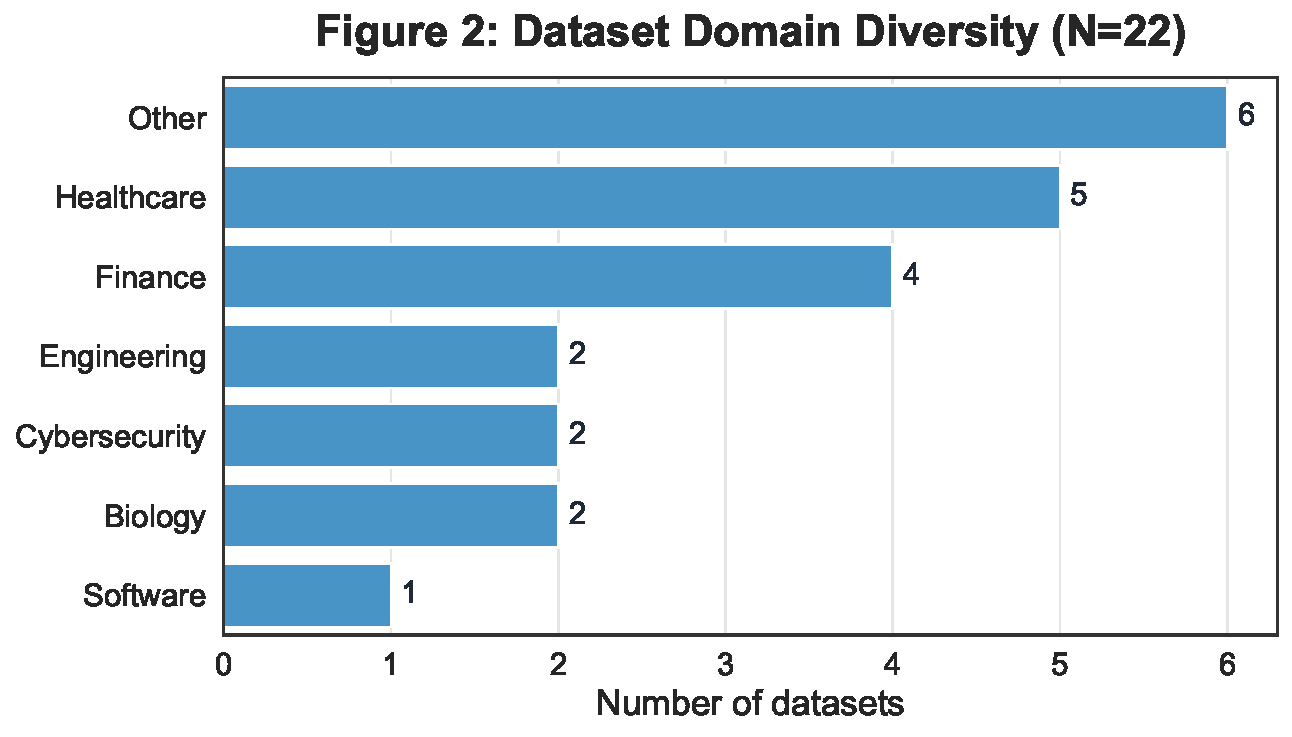
\includegraphics[width=0.92\linewidth]{Figure_2_Dataset_Diversity.pdf}
\caption{Domain composition of the 22-dataset primary analysis scope.}
\label{fig:diversity}
\end{figure}

\subsection{Task design}
Each data set is evaluated with seeds $\{42,123,456,789,2025\}$ and five folds.  The configured conditions are clean training data; Gaussian noise with standard deviations 0.01, 0.05, and 0.10; missing values at rates 0.05, 0.10, and 0.20; label noise at rates 0.05, 0.10, and 0.20; covariate partitioning; feature removal at 0.20; population partitioning; and class-prior relabeling.  The perturbations are applied to the training partition; the held-out test partition remains clean.  Consequently, the robustness analysis is about corrupted training data, not a direct test-time deployment-shift experiment.

For data set $d$, seed $s$, fold $f$, condition $c$, pipeline $p$, and classifier $m$, write the clean sample as
\begin{equation}
  D_d=\{(x_i,y_i)\}_{i=1}^{n_d}=T_{d s f}\,\dot\cup\,V_{d s f},
\end{equation}
where $T$ is the training partition and $V$ is the held-out partition.  A condition is an operator $\Pi_c$ with a recorded random state $\xi_{sfc}$, so the fitted training sample is $\widetilde T_{d s f c}=\Pi_c(T_{d s f};\xi_{sfc})$, while $V_{d s f}$ is unchanged.  The fold-local preprocessing and feature map are denoted by $\phi_{p d s f}$, and the fitted predictor is
\begin{equation}
  \widehat f_{p m d s f c}=\operatorname{Fit}_{m}\!\left(\phi_{p d s f}(\widetilde T_{d s f c})\right).
\end{equation}
This notation makes explicit that the benchmark estimates a conditional quantity, $\operatorname{Perf}(\widehat f;\,\Pi_c(T),V)$, rather than performance on a shifted test population.

The ordinary splitter uses stratified five-fold partitioning and falls back to a regular K-fold splitter when a class has fewer than five observations.  Covariate and population partitions use global data-frame representations before the fold-local preprocessing stage.  This implementation detail means that those two conditions should be treated as stress tests rather than as leakage-free estimates of deployment shift.

\subsection{Pipelines and estimators}
The seven pipelines are Raw, Raw\_Variance, Raw\_MI, AutoFE\_Baseline, AutoFE\_MI, AutoFE\_Random, and AutoFE\_NoMultiply.  Every pipeline first retains at most 20 preprocessed columns using a variance-ranked stage.  Thus the three names beginning with Raw are capped raw-feature baselines and are intentionally not full-dimensional raw-data controls.  DFS uses depth-one arithmetic primitives.  The NoMultiply variant removes both multiplication and division, leaving addition and subtraction; the name should not be read as removing multiplication alone.

The estimator menu contains logistic regression, random forest, ExtraTrees, XGBoost \citep{chen2016}, LightGBM \citep{ke2017}, CatBoost \citep{prokhorenkova2018}, a calibrated linear SVM, five-nearest-neighbour classification, Gaussian naive Bayes, and a one-hidden-layer multilayer perceptron.  Numeric variables are imputed and standardized; categorical variables are imputed and one-hot encoded with unknown-category handling, following the conventional scikit-learn-style preprocessing stack \citep{pedregosa2011}.  Feature generation and preprocessing are performed within the recorded fold task, but the benchmark does not store complete data/code/library provenance for every checkpoint.

Let $X^{(0)}$ denote the encoded fold-local matrix.  The retained raw representation is
\begin{equation}
  X^{\mathrm{raw}}=X^{(0)}_{[:,\,\operatorname{Top}_{20}(\operatorname{Var}(X^{(0)}))]}.
\end{equation}
For AutoFE, the depth-one candidate set is
\begin{equation}
  \mathcal{G}(X^{(0)})=\left\{x_i+x_j,\ x_i-x_j,\ x_i\times x_j,\ x_i/x_j:\ i,j\in\{1,\ldots,p\}\right\},
\end{equation}
subject to finite-value checks and the runner’s feature cap.  AutoFE\_Baseline ranks candidates by variance, AutoFE\_MI by mutual information, AutoFE\_Random by a deterministic averaged random score, and AutoFE\_NoMultiply removes both $\times$ and $/$ from $\mathcal{G}$.  The final design matrix is a selected union of raw and generated columns, capped at 100 columns for AutoFE variants.  This formalization explains why the experiment tests search-space control, not an unconstrained universal feature learner.

\subsection{Recorded outcomes and analysis}
The result ledger records ROC--AUC, PR--AUC, accuracy, F1, log loss, Brier score, train/test AUC, Kolmogorov--Smirnov and Wasserstein distances, feature counts, resident-memory deltas, and feature-generation, training, and inference times.  Non-finite values occur in the JSONL ledger as the non-standard token \texttt{NaN}; they are excluded metric-by-metric rather than imputed.  Multiclass PR--AUC is frequently unavailable, and the implementation’s Brier-score label handling is not valid for all multiclass cases.  Accordingly, ROC--AUC is the primary comparative endpoint; calibration metrics are treated as diagnostic outputs.

We summarize means over available task records, train--test AUC gaps, and condition-wise means.  Pairwise higher/equal/lower counts are retained as descriptive checks.  A confirmatory submission should replace pooled row-level tests with a hierarchical analysis at the data-set/fold level and apply an explicit multiplicity correction; the original pooled Wilcoxon and Friedman outputs are not treated as proof of universal superiority or inferiority.

\subsection{Estimands and aggregation}
For a binary held-out fold with score $r_i=\widehat f(x_i)$, ROC--AUC is the probability that a randomly selected positive receives a larger score than a randomly selected negative, with half credit for ties \citep{fawcett2006}:
\begin{equation}
  \widehat{\AUC}_{pmdsfc}=\frac{1}{|V^+||V^-|}
  \sum_{i\in V^+}\sum_{j\in V^-}
  \left[\mathbb{1}(r_i>r_j)+\tfrac12\mathbb{1}(r_i=r_j)\right].
\end{equation}
The train--test gap is
\begin{equation}
  \Delta_{pmdsfc}=\widehat{\AUC}^{\mathrm{train}}_{pmdsfc}-\widehat{\AUC}^{\mathrm{test}}_{pmdsfc},
\end{equation}
and the condition-wise robustness ratio is
\begin{equation}
  R_{p,c}=\frac{\E_{d,s,f,m}[\widehat{\AUC}_{p m d s f c}\mid c]}{\E_{d,s,f,m}[\widehat{\AUC}_{p m d s f,\mathrm{clean}}]}.
\end{equation}
For computational cost, the recorded wall-clock decomposition is
\begin{equation}
  T^{\mathrm{total}}=T^{\mathrm{FE}}+T^{\mathrm{fit}}+T^{\mathrm{infer}},
  \qquad
  \rho_{p}=\frac{n^{\mathrm{retained}}_{p}}{n^{\mathrm{original}}_{p}},
\end{equation}
where $n^{\mathrm{original}}$ is the post-one-hot dimension stored by the runner, not necessarily the source-table column count.

The result ledger is a task-level sample and is unbalanced after interruption.  We therefore report both the task-row mean and a data-set-balanced sensitivity estimate.  For metric $z$, let $I_{dp}$ be the available rows for data set $d$ and pipeline $p$; then
\begin{equation}
  \overline z_{dp}=\frac{1}{|I_{dp}|}\sum_{i\in I_{dp}}z_i,
  \qquad
  \widehat\mu^{\mathrm{DS}}_p=\frac{1}{|D_p|}\sum_{d\in D_p}\overline z_{dp}.
\end{equation}
The uncertainty bars in the data-set-balanced table are descriptive normal-approximation intervals $\widehat\mu^{\mathrm{DS}}_p\pm1.96\,s_p/\sqrt{|D_p|}$, with $s_p$ the standard deviation of the 22 data-set means.  This is not a substitute for a mixed-effects model, but it prevents the large data sets and dense task blocks from silently receiving extra weight.

\subsection{Completion and censoring accounting}
The intended experiment size is
\begin{equation}
  N_{\mathrm{grid}}=25\times5\times5\times14\times7\times10=612{,}500.
\end{equation}
The primary JSONL ledger contains $N_{\mathrm{success}}=560{,}002$ completed evaluation rows, giving a nominal completion fraction $C=91.43\%$.  The 22-dataset scope contains 538,972 rows out of 539,000 possible rows ($99.995\%$), with the small deficit confined to the two near-complete data sets.  No failed task is represented as a row with a failure status: worker exceptions are logged separately and the checkpoint database records completed task hashes.  We therefore treat the observed ledger as right-censored by completion, not as a missing-at-random sample.  The stopping rule was computational: the final large-data blocks contained linear-model tasks with multi-hour tails, and the runs were stopped after the completed evidence was sufficient to estimate the primary ordering.  This decision is scientifically transparent, but it limits claims about the three uncompleted data sets.

\section{Theoretical framework: Feature-Synthesis Variance Amplification}
\label{sec:theory}

The empirical pattern motivates a mechanistic contribution.  We define the \emph{Feature-Synthesis Variance Amplification (FSVA) effect} as the regime in which perturbation amplification, estimation variance, and search multiplicity outweigh the approximation-bias reduction supplied by a generated representation.  This definition does not assert that all feature engineering fails.  It specifies mechanisms and falsifiable predictions for the regime in which the variance and perturbation penalties exceed the reduction in approximation bias.

The following dimensionless index is the paper's compact summary of that mechanism.  Let $r$ be the capped raw-feature reference, let $\tau>0$ be a small numerical floor, let $\mathcal{V}_p$ denote an estimation-variance proxy derived from Eq.~\eqref{eq:coef_var}, let $M_p$ be the effective candidate count, and let $\mathcal{B}_p$ be the non-negative approximation-bias term in Eq.~\eqref{eq:risk_decomp}:
\begin{equation}
\boxed{\begin{aligned}
  \Phi_{\mathrm{FSVA}}(p\mid r)
  &=\underbrace{A_p}_{\text{perturbation amplification}}
   +\underbrace{V_p}_{\text{variance inflation}}
   +\underbrace{S_p}_{\text{search multiplicity}}
   -\underbrace{B_p}_{\text{bias reduction}},\\[-2pt]
  A_p&=\log\!\frac{\operatorname{tr}\!\left(J_{g_p}\Sigma_{\varepsilon}J_{g_p}^{\mathsf T}\right)+\tau}
                         {\operatorname{tr}(\Sigma_{\varepsilon})+\tau},\quad
  V_p=\log\!\frac{\mathcal{V}_p+\tau}{\mathcal{V}_r+\tau},\quad
  S_p=\log\!\frac{M_p+\tau}{M_r+\tau},\quad
  B_p=\log\!\frac{\mathcal{B}_r+\tau}{\mathcal{B}_p+\tau}.
\end{aligned}}
\label{eq:fsva_master}
\end{equation}
All four terms are log ratios relative to the same reference and are therefore dimensionless.  A positive $\Phi_{\mathrm{FSVA}}$ means that the aggregate amplification, variance, and search penalties exceed the bias reduction; a negative value means that the representation's bias reduction dominates.  The current ledger directly supports the observable implications of these terms, but it does not contain every latent quantity, such as Jacobian norms or candidate-level selection histories.  We therefore use Eq.~\eqref{eq:fsva_master} as a mechanistic accounting identity and falsifiable design target, not as a post hoc fitted score.

\subsection{Error propagation through generated operators}
Let $g:\mathbb{R}^{p}\rightarrow\mathbb{R}^{q}$ map an encoded base vector $x$ to generated features and let $\varepsilon$ be a zero-mean training perturbation with covariance $\Sigma_{\varepsilon}$.  If $g$ is twice differentiable in a neighborhood of $x$ and has bounded Hessian, a first-order Taylor expansion gives
\begin{equation}
  g(x+\varepsilon)-g(x)=J_g(x)\varepsilon+r(x,\varepsilon),
  \qquad \|r(x,\varepsilon)\|=O(\|\varepsilon\|^2),
\end{equation}
where $J_g(x)$ is the $q\times p$ Jacobian.  Taking the conditional second moment yields
\begin{equation}
  \mathbb{E}\!\left[\|g(x+\varepsilon)-g(x)\|_2^2\mid x\right]
  =\operatorname{tr}\!\left(J_g(x)\Sigma_{\varepsilon}J_g(x)^{\mathsf T}\right)
  +O\!\left(\mathbb{E}\|\varepsilon\|_2^3\right).
  \label{eq:jacobian_amp}
\end{equation}
Equation~\eqref{eq:jacobian_amp} is the core FSVA quantity.  The raw representation has $J_g=I$; an operator is locally variance-amplifying when the trace on the right exceeds $\operatorname{tr}(\Sigma_{\varepsilon})$.  The benchmark does not record $J_g$ directly, so this quantity is a theoretical diagnostic and a concrete target for the next implementation revision.

\paragraph{Proof sketch.} Substitute the Taylor expansion into the squared norm, take expectations, and use $\mathbb{E}[\varepsilon]=0$ to eliminate the first-order cross term.  The remaining quadratic term is $\mathbb{E}[\varepsilon^{\mathsf T}J_g^{\mathsf T}J_g\varepsilon]=\operatorname{tr}(J_g\Sigma_{\varepsilon}J_g^{\mathsf T})$; bounded second derivatives control the remainder by the third moment of $\varepsilon$.  The result is local, but it is exact for affine maps and gives the leading term for the arithmetic primitives used here.

For the product primitive $g(x_a,x_b)=x_a x_b$, the perturbation is exact:
\begin{equation}
  \delta g=x_a\varepsilon_b+x_b\varepsilon_a+\varepsilon_a\varepsilon_b.
\end{equation}
With independent zero-mean perturbations of variances $\sigma_a^2$ and $\sigma_b^2$,
\begin{equation}
  \operatorname{Var}(\delta g\mid x)
  =x_b^2\sigma_a^2+x_a^2\sigma_b^2+\sigma_a^2\sigma_b^2.
  \label{eq:product_amp}
\end{equation}
Thus a large-magnitude companion feature magnifies noise in the other feature, and the quadratic term remains even when the observed feature values are small.  For the division primitive $g(x_a,x_b)=x_a/x_b$, the local approximation is
\begin{equation}
  \operatorname{Var}(\delta g\mid x)\approx
  \frac{\sigma_a^2}{x_b^2}+\frac{x_a^2\sigma_b^2}{x_b^4},
  \label{eq:ratio_amp}
\end{equation}
which becomes arbitrarily large as $|x_b|\rightarrow0$.  Missing-value imputation, label-dependent partitioning, and finite-value filtering may truncate these tails in practice, but they do not remove the underlying sensitivity.  Equations~\eqref{eq:product_amp}--\eqref{eq:ratio_amp} provide a direct explanation for why unrestricted multiplication/division can be more fragile than an addition/subtraction-only search.

\subsection{Variance inflation and redundancy}
Suppose the learner receives a design matrix $Z_p$ containing raw and generated columns and uses a ridge-stabilized linear fit with penalty $\lambda$.  For the model $y=Z_p\beta+\eta$, $\operatorname{Var}(\eta)=\sigma_y^2I$, the conditional covariance of the fitted coefficient vector is \citep{hastie2009,zou2005}
\begin{equation}
  \operatorname{Var}(\widehat\beta_{p,\lambda}\mid Z_p)
  =\sigma_y^2 A_{p,\lambda}Z_p^{\mathsf T}Z_pA_{p,\lambda},
  \qquad A_{p,\lambda}=(Z_p^{\mathsf T}Z_p+\lambda I)^{-1}.
  \label{eq:coef_var}
\end{equation}
When generated columns are nearly redundant, the smallest eigenvalues of $Z_p^{\mathsf T}Z_p$ approach zero and the unregularized covariance in Eq.~\eqref{eq:coef_var} inflates.  A useful complexity measure is the ridge effective degrees of freedom
\begin{equation}
  \operatorname{df}_{\lambda}(Z_p)=\operatorname{tr}\!\left[Z_p(Z_p^{\mathsf T}Z_p+\lambda I)^{-1}Z_p^{\mathsf T}\right]
  =\sum_{j}\frac{s_j^2}{s_j^2+\lambda},
  \label{eq:effective_df}
\end{equation}
where $s_j$ are singular values of $Z_p$.  The number of stored columns can grow while the effective rank remains almost unchanged; in that case the representation pays a conditioning and search cost without buying independent signal.  The effective-rank diagnostic
\begin{equation}
  r_{\mathrm{eff}}(\Gamma)=\frac{\operatorname{tr}(\Gamma)^2}{\operatorname{tr}(\Gamma^2)}
\end{equation}
quantifies this distinction for feature covariance $\Gamma$.  A large column count together with a small $r_{\mathrm{eff}}$ is the signature of redundant feature synthesis rather than genuine representational expansion.

\subsection{Search multiplicity and the bias--variance crossover}
Even if every candidate feature is conditionally independent of the label, selecting the best-looking candidate over $M$ trials creates a selection effect.  For standardized sub-Gaussian null scores $S_j$ based on $n$ observations, the usual extreme-value approximation is
\begin{equation}
  \mathbb{E}\left[\max_{1\le j\le M}|S_j|\right]
  \approx \sigma_S\sqrt{2\log M},
  \qquad \sigma_S=O(n^{-1/2}).
  \label{eq:search_max}
\end{equation}
The depth-one arithmetic library grows approximately quadratically in the number of encoded columns before filtering.  Consequently, the selection threshold can increase even when the data contain no additional signal.  Mutual-information and randomized rankings change which candidates survive, but they do not eliminate the multiplicity term in Eq.~\eqref{eq:search_max}.

Equation~\eqref{eq:search_max} is an asymptotic diagnostic under standardized, sub-Gaussian null scores; it is not used to assign a numerical penalty to the current results.  Its role is to make the selection mechanism explicit and to identify the candidate count and fold-wise selection history as quantities that a future implementation must record.

For a predictor trained on representation $p$, the expected test risk can be written schematically as \citep{hastie2009,belkin2019}
\begin{equation}
  \mathcal{R}_p
  =\underbrace{\sigma_{\mathrm{irr}}^2}_{\text{irreducible noise}}
  +\underbrace{\operatorname{Bias}_p^2}_{\text{approximation error}}
  +\underbrace{\operatorname{Var}_p}_{\text{estimation/search variance}}
  +\underbrace{\mathcal{A}_p(\Sigma_{\varepsilon})}_{\text{perturbation amplification}},
  \label{eq:risk_decomp}
\end{equation}
where $\mathcal{A}_p$ is induced by Eq.~\eqref{eq:jacobian_amp}.  Relative to a capped raw representation $r$, feature synthesis is beneficial only when
\begin{equation}
  \operatorname{Bias}_{r}^{2}-\operatorname{Bias}_{p}^{2}
  >\left(\operatorname{Var}_{p}-\operatorname{Var}_{r}\right)
   +\left(\mathcal{A}_{p}-\mathcal{A}_{r}\right).
  \label{eq:crossover}
\end{equation}
The FSVA regime is the opposite inequality.  The inequality specifies the competition between approximation benefit, conditioning and search variance, and operator sensitivity.

\begin{table}[H]
\centering
\small
\caption{FSVA mechanisms, empirical predictions, and evidence in the present benchmark.}
\label{tab:fsva}
\begin{tabular}{p{0.24\linewidth}p{0.33\linewidth}p{0.31\linewidth}}
\toprule
Mechanism & Falsifiable prediction & Evidence in the completed scope \\
\midrule
Jacobian amplification & Product/division operators should show larger degradation under training perturbations than addition/subtraction operators. & Clean-to-0.20 missingness decline: 0.0756 for AutoFE\_Baseline versus 0.0083 for AutoFE\_NoMultiply. \\
Redundancy and conditioning & Broad synthesis should increase feature complexity and train--test separation without a commensurate test-AUC gain. & AutoFE\_Baseline gap 0.1181 versus 0.0701 for Raw; runtime and feature-complexity panels show the associated cost. \\
Search multiplicity & Larger candidate libraries should produce larger apparent training gains and greater sensitivity to selection randomness. & AutoFE\_Random and AutoFE\_MI remain between the raw reference and unrestricted baseline, rather than uniformly improving it. \\
Bias--variance crossover & An operator restriction can recover performance if it removes variance/amplification faster than it removes useful signal. & AutoFE\_NoMultiply reaches mean ROC--AUC 0.8237 versus 0.8263 for Raw. \\
\bottomrule
\end{tabular}
\end{table}

The table is a theory-to-evidence map, not a post hoc proof of every latent quantity.  In particular, the current ledger does not contain Jacobian norms, singular spectra, or candidate-level selection histories.  These measurements are the most direct falsification tests for FSVA and define a concrete software extension for a revision or follow-up study.

\section{Results}
\label{sec:results}

\subsection{Predictive performance}
Table~\ref{tab:roc} reports mean ROC--AUC in the primary scope.  The capped raw-feature pipelines consistently achieved higher predictive performance than the broad synthesis variants, while the three raw-feature controls were numerically indistinguishable.  AutoFE\_NoMultiply remained close to the raw-feature reference, whereas the broader synthesis/selection variants were lower.

\begin{table}[t]
\centering
\caption{Mean ROC--AUC across the 22-dataset primary scope.  Values are descriptive means over available successful task records.}
\label{tab:roc}
\begin{tabular}{lcc}
\toprule
Pipeline & Mean ROC--AUC & Difference from Raw \\
\midrule
Raw & 0.8263 & 0.0000 \\
Raw\_Variance & 0.8263 & $-0.0000$ \\
Raw\_MI & 0.8262 & $-0.0001$ \\
AutoFE\_NoMultiply & 0.8237 & $-0.0026$ \\
AutoFE\_MI & 0.7985 & $-0.0278$ \\
AutoFE\_Random & 0.7804 & $-0.0459$ \\
AutoFE\_Baseline & 0.7481 & $-0.0782$ \\
\bottomrule
\end{tabular}
\end{table}

\begin{table}[t]
\centering
\caption{Data-set-balanced ROC--AUC sensitivity analysis.  The mean is the arithmetic mean of the 22 data-set means; the interval is descriptive $95\%$ normal approximation across data sets.}
\label{tab:balanced}
\begin{tabular}{lccc}
\toprule
Pipeline & Mean & Across-data-set SD & Descriptive 95\% interval \\
\midrule
Raw & 0.8262 & 0.1140 & [0.7785, 0.8738] \\
Raw\_Variance & 0.8261 & 0.1140 & [0.7785, 0.8738] \\
Raw\_MI & 0.8261 & 0.1140 & [0.7785, 0.8738] \\
AutoFE\_NoMultiply & 0.8237 & 0.1142 & [0.7759, 0.8714] \\
AutoFE\_MI & 0.7984 & 0.1198 & [0.7484, 0.8485] \\
AutoFE\_Random & 0.7803 & 0.1128 & [0.7332, 0.8274] \\
AutoFE\_Baseline & 0.7476 & 0.1124 & [0.7006, 0.7945] \\
\bottomrule
\end{tabular}
\end{table}

The balanced estimate changes the fourth decimal place but not the ordering, which is important because the interrupted ledger contains unequal block lengths.  Relative to the raw-feature reference, the balanced penalties are 9.5\% for AutoFE\_Baseline, 5.5\% for AutoFE\_Random, 3.4\% for AutoFE\_MI, and 0.3\% for AutoFE\_NoMultiply.  At the data-set level, the raw-feature mean is higher than AutoFE\_Baseline on all 22 data sets (mean paired difference $0.0786$, SD $0.0623$, descriptive 95\% interval $[0.0526,0.1046]$).  The raw-feature mean is also higher than AutoFE\_Random on all 22 and higher than AutoFE\_MI on 21 of 22.  AutoFE\_NoMultiply is the genuinely close comparison: the raw-feature mean is higher on 14 data sets and lower on 8, with mean difference $0.0025$ (SD $0.0066$, interval $[-0.0002,0.0053]$).  These data-set-level contrasts are stronger evidence than a pooled row count because each data set contributes one mean to the sensitivity analysis.

Figure~\ref{fig:workflow} shows the benchmark execution and publication path.  Figure~\ref{fig:pipeline} provides the regenerated ranking.  The ordering is not a claim about all AutoFE systems: it is the ordering produced by this operator set, feature cap, estimator menu, and training-corruption design.

\begin{figure}[H]
\centering
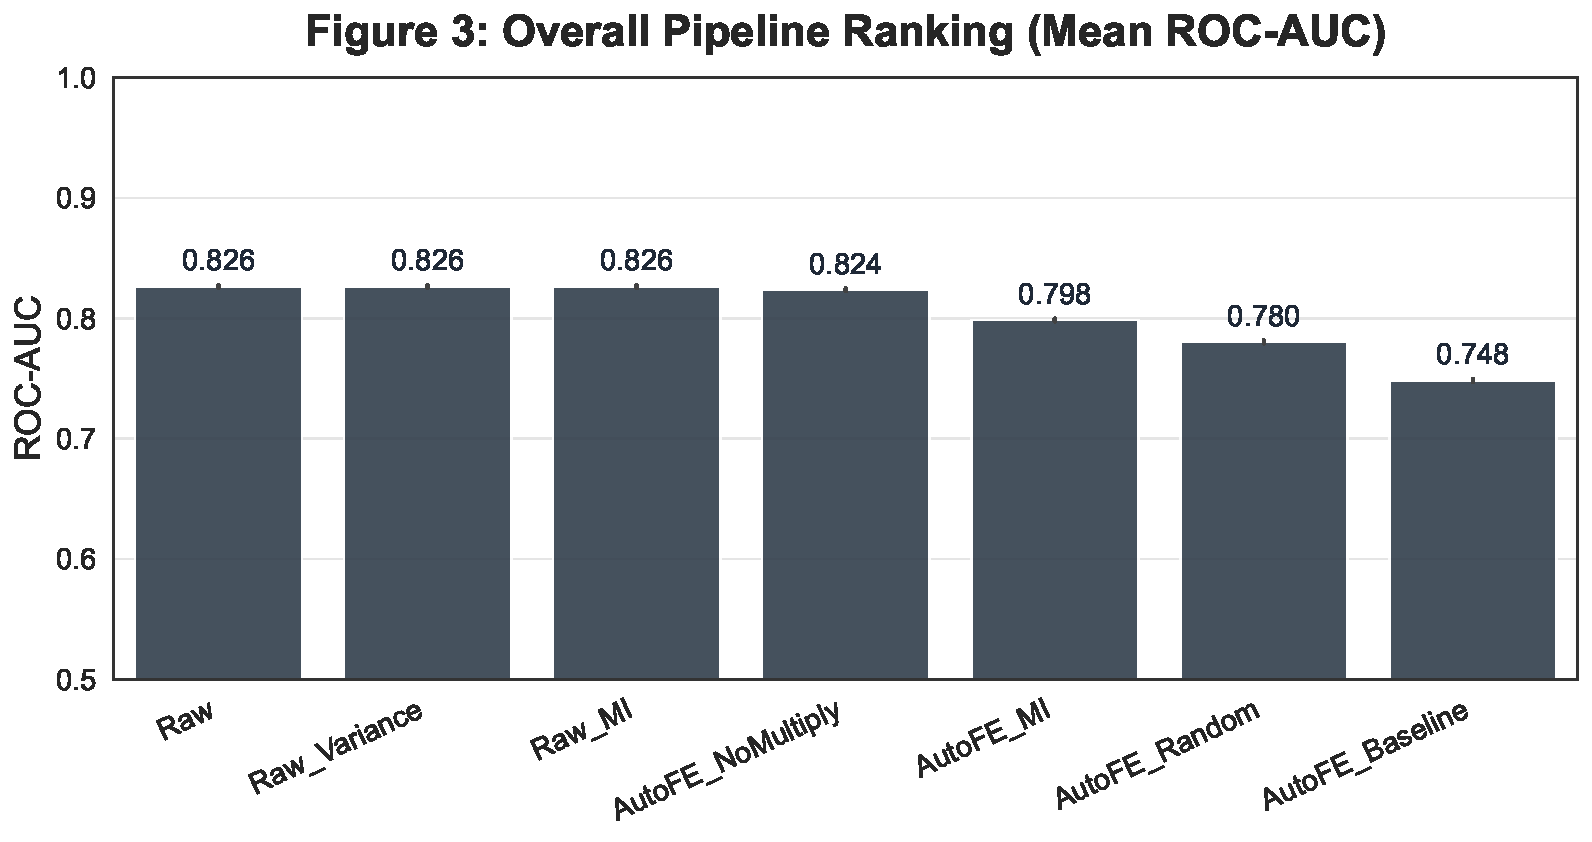
\includegraphics[width=0.92\textwidth]{Figure_3_Pipeline_Ranking.pdf}
\caption{Regenerated mean ROC--AUC ranking for the seven pipelines in the primary scope.}
\label{fig:pipeline}
\end{figure}

The pipeline ordering is not driven by one classifier family alone.  Figure~\ref{fig:models} shows the corresponding classifier-level performance across the same conditions and pipeline menu; this provides a model-side check before attributing the result to feature construction.

\begin{figure}[H]
\centering
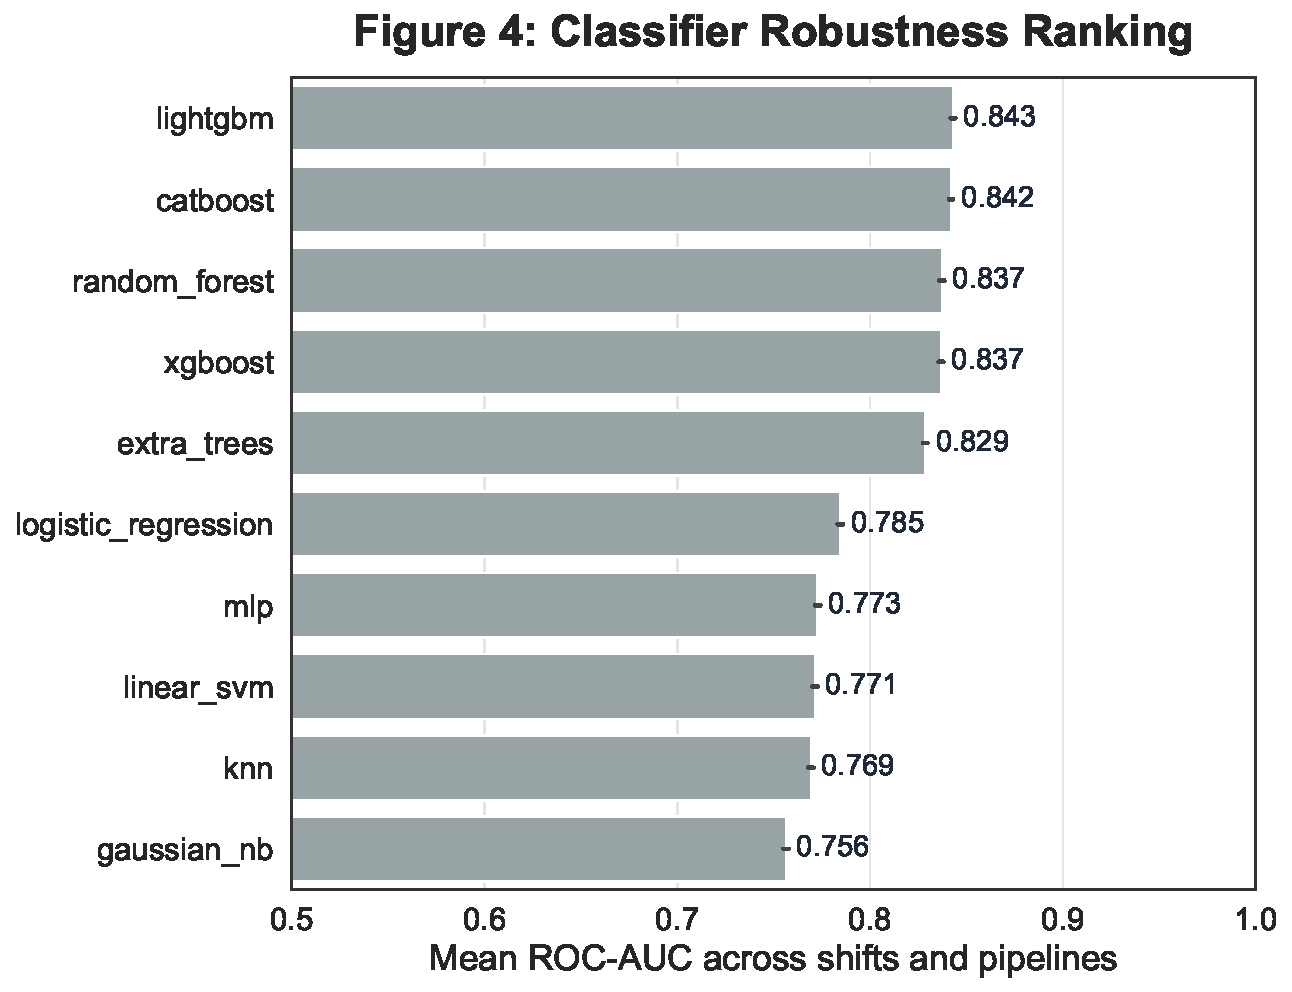
\includegraphics[width=0.92\linewidth]{Figure_4_Model_Ranking.pdf}
\caption{Classifier-level mean ROC--AUC across the evaluated pipelines and training-data conditions.}
\label{fig:models}
\end{figure}

\subsection{Training-data corruption and train--test gaps}
Across the 22-dataset scope, clean-condition mean ROC--AUC is 0.8488 for Raw and 0.7874 for AutoFE\_Baseline.  At missingness rates 0.05, 0.10, and 0.20, the corresponding Raw values are 0.8476, 0.8455, and 0.8415, while AutoFE\_Baseline obtains 0.7241, 0.7223, and 0.7118.  Under covariate and population partitioning, Raw obtains 0.7403 and 0.7525, compared with 0.6845 and 0.6955 for AutoFE\_Baseline.  These are training-corruption stress results because the test data were not shifted.

The mean train--test AUC gap increases from approximately 0.0701 for Raw to 0.0756 for AutoFE\_NoMultiply, 0.0823 for AutoFE\_MI, 0.0932 for AutoFE\_Random, and 0.1181 for AutoFE\_Baseline.  The gap is consistent with, but does not by itself prove, a feature-synthesis overfitting mechanism.  The regenerated robustness and ablation figures are supplied as supporting diagnostics (Figures~\ref{fig:robustness} and~\ref{fig:ablation}).

\begin{table}[t]
\centering
\small
\caption{Condition-wise mean ROC--AUC for three representative pipelines in the 22-dataset scope.  Conditions perturb training data; the held-out test partition is unchanged.}
\label{tab:conditions}
\begin{tabular}{lrrr}
\toprule
Condition & Raw & AutoFE\_Baseline & AutoFE\_NoMultiply \\
\midrule
clean & 0.8488 & 0.7874 & 0.8475 \\
gaussian noise 0.01 & 0.8498 & 0.7822 & 0.8486 \\
gaussian noise 0.05 & 0.8482 & 0.7752 & 0.8469 \\
gaussian noise 0.10 & 0.8475 & 0.7691 & 0.8460 \\
missing values 0.05 & 0.8476 & 0.7241 & 0.8465 \\
missing values 0.10 & 0.8455 & 0.7223 & 0.8438 \\
missing values 0.20 & 0.8415 & 0.7118 & 0.8392 \\
label noise 0.05 & 0.8404 & 0.7750 & 0.8381 \\
label noise 0.10 & 0.8311 & 0.7655 & 0.8294 \\
label noise 0.20 & 0.8075 & 0.7359 & 0.8037 \\
feature removal 0.20 & 0.8388 & 0.7915 & 0.8380 \\
class-prior relabeling & 0.7993 & 0.7325 & 0.7981 \\
covariate partition & 0.7403 & 0.6845 & 0.7316 \\
population partition & 0.7525 & 0.6955 & 0.7429 \\
\bottomrule
\end{tabular}
\end{table}

The broad baseline is particularly sensitive to missingness: its AUC falls by 0.0756 between the clean and 0.20-missing conditions, compared with 0.0073 for Raw and 0.0083 for AutoFE\_NoMultiply.  The result is consistent with error propagation through arithmetic features, but the experiment does not identify which individual primitive caused the loss.  The covariate/population rows are the lowest-performing conditions for every pipeline, supporting the narrower conclusion that these partitions are difficult stress tests rather than evidence of deployment robustness.

\begin{figure}[H]
\centering
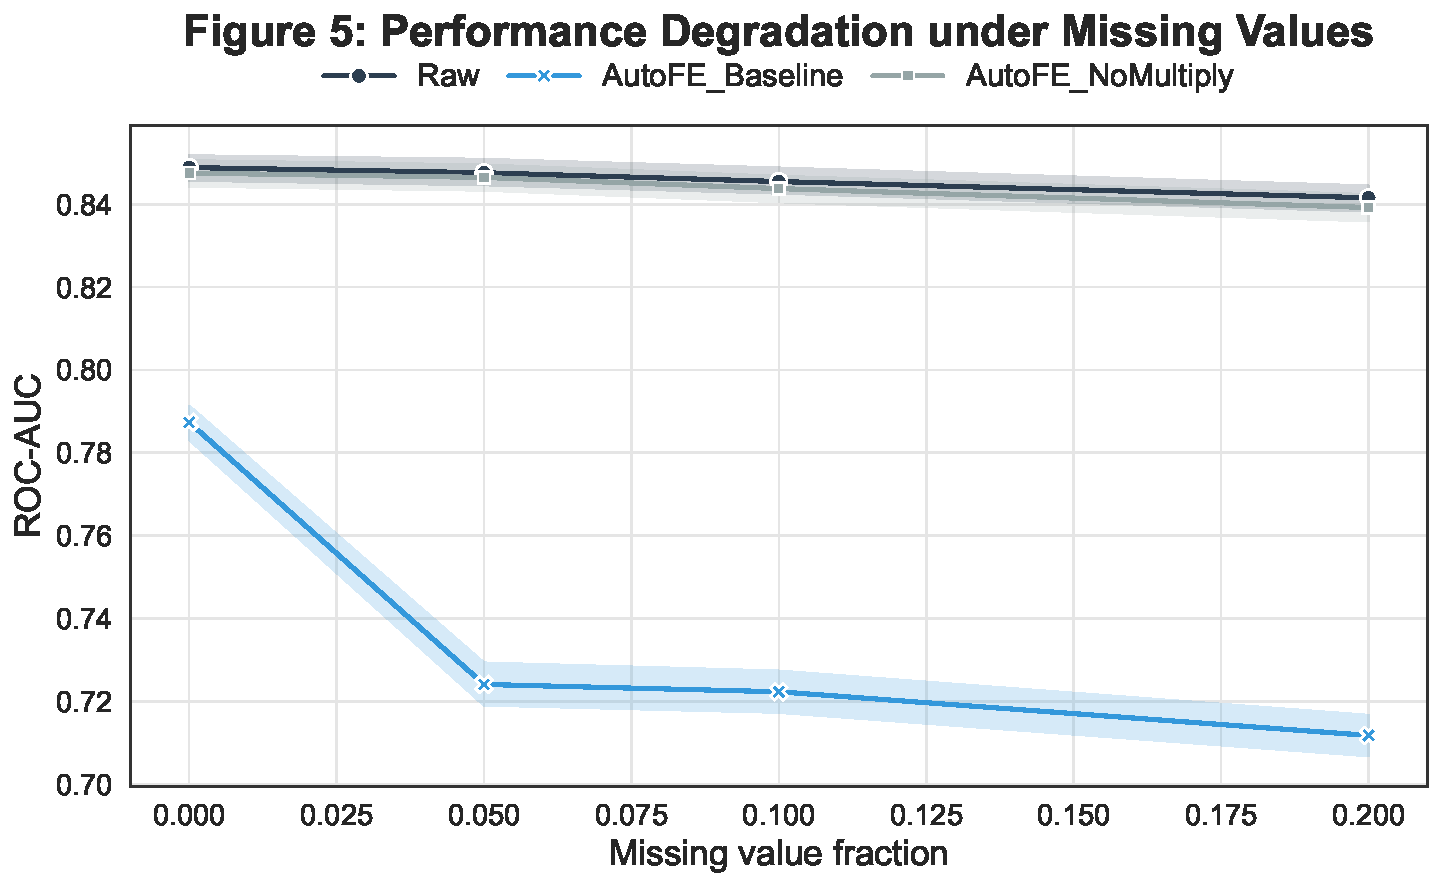
\includegraphics[width=0.92\textwidth]{Figure_5_Robustness_Shift.pdf}
\caption{Mean ROC--AUC by training-data corruption condition in the primary scope.}
\label{fig:robustness}
\end{figure}

\subsection{Computational cost and feature complexity}
In the primary 22-dataset records, median feature-generation/training/inference times are 0.003/0.138/0.007 seconds for Raw, 0.614/0.455/0.012 for AutoFE\_Baseline, 4.387/0.346/0.012 for AutoFE\_MI, 0.283/0.272/0.012 for AutoFE\_NoMultiply, and 0.563/0.408/0.012 for AutoFE\_Random.  These medians summarize completed rows; they do not represent a hardware-normalized energy study.  The largest observed training-time outlier is approximately 37,569 seconds (10.4 hours) for a linear SVM task on \texttt{kddcup99}, which explains why the final large-data blocks were not allowed to run indefinitely.

Figure~\ref{fig:runtime} places the three timing components on a common logarithmic axis.  The visual separation is substantive: feature generation dominates the AutoFE\_MI and AutoFE\_Baseline medians, while the capped raw variants have no comparable synthesis stage.

\begin{figure}[H]
\centering
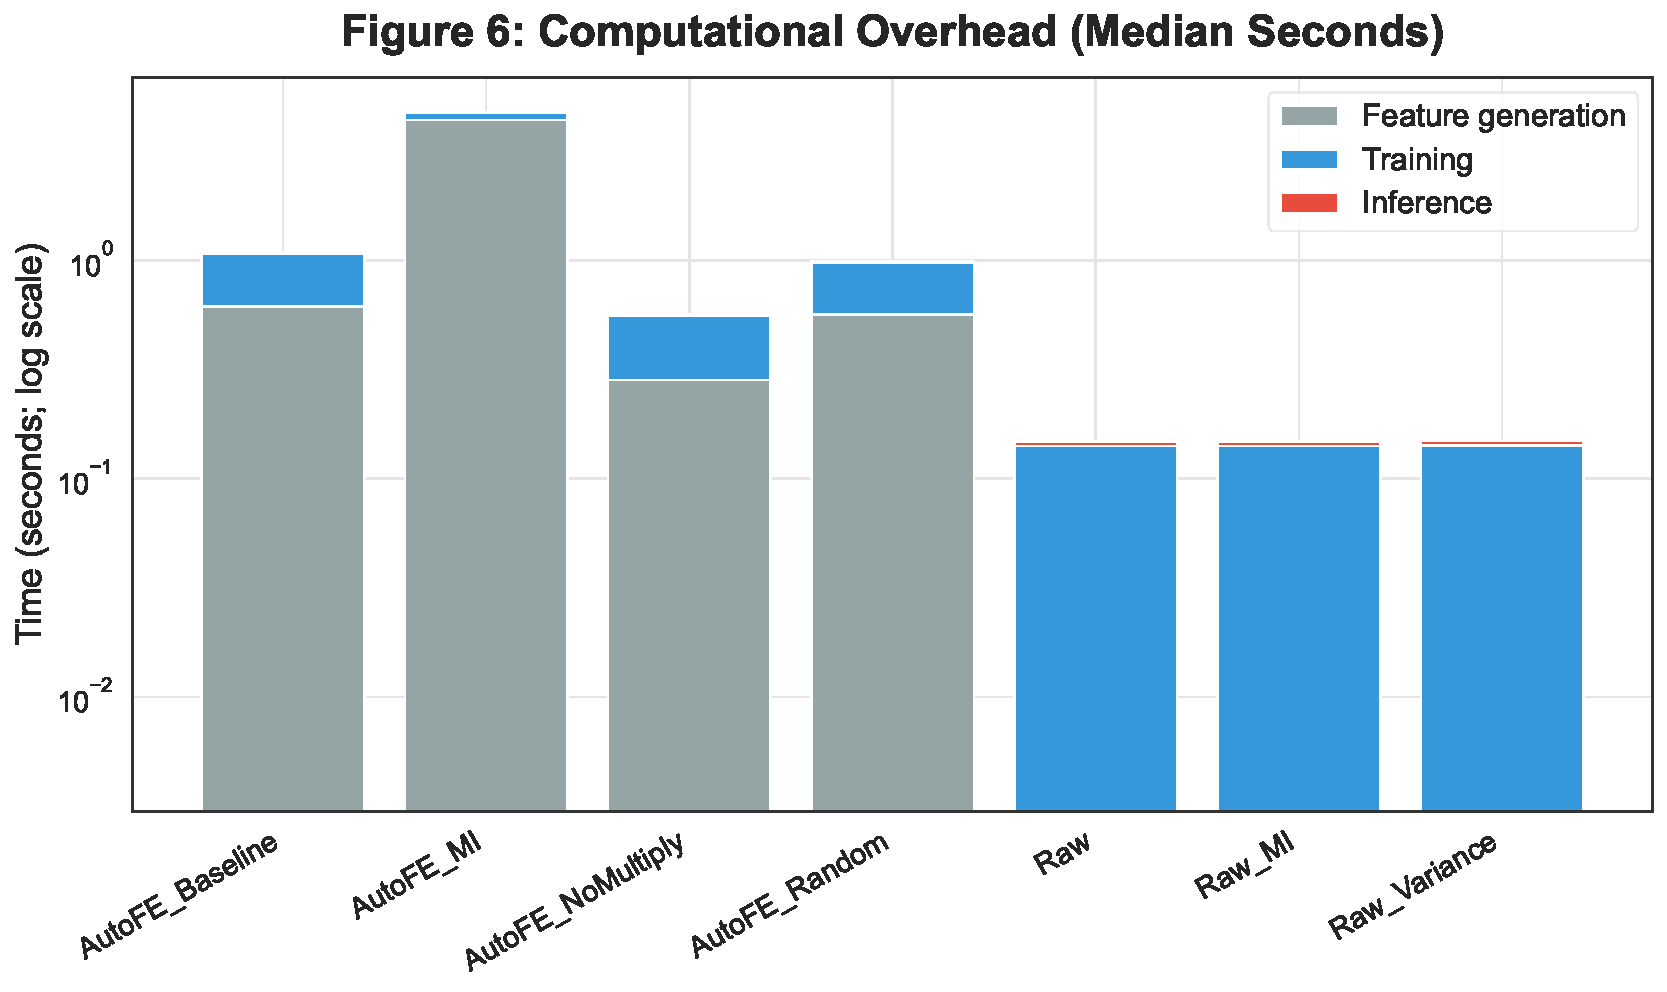
\includegraphics[width=0.94\linewidth]{Figure_6_Runtime_Comparison.pdf}
\caption{Median feature-generation, training, and inference time by pipeline.  The logarithmic axis preserves both sub-second raw baselines and multi-second synthesis costs.}
\label{fig:runtime}
\end{figure}

AutoFE variants also produce larger intermediate representations and resident-memory deltas than the capped raw baselines.  Figure~\ref{fig:complexity} reports the regenerated feature-complexity view.  Because the stored \texttt{n\_original} field is post-one-hot dimensionality and \texttt{ram\_used\_mb} is a process RSS delta, these fields should not be interpreted as exact source-column counts or peak physical memory.

\begin{figure}[H]
\centering
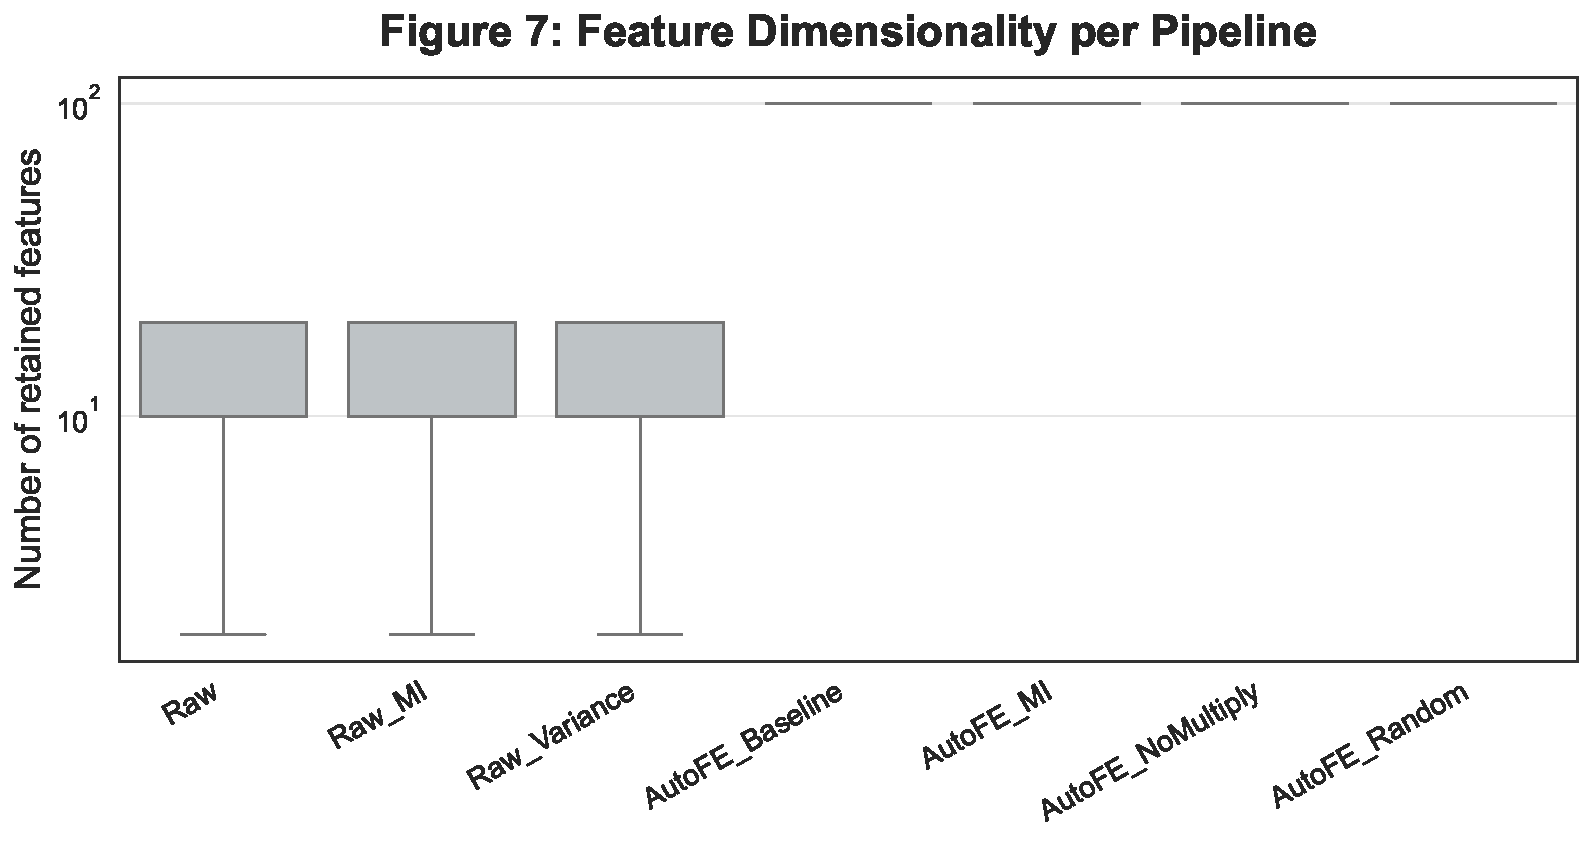
\includegraphics[width=0.92\textwidth]{Figure_7_Feature_Complexity.pdf}
\caption{Feature dimensionality and recorded complexity measures.}
\label{fig:complexity}
\end{figure}

The operator ablation in Figure~\ref{fig:ablation} closes the cost--accuracy loop.  Removing multiplication and division recovers nearly the raw-feature ROC--AUC while avoiding the broadest candidate expansion; mutual-information and randomized selection occupy intermediate positions.  The result is evidence for an operator-sensitive design principle, not a claim that addition and subtraction are optimal for every domain.

\begin{figure}[H]
\centering
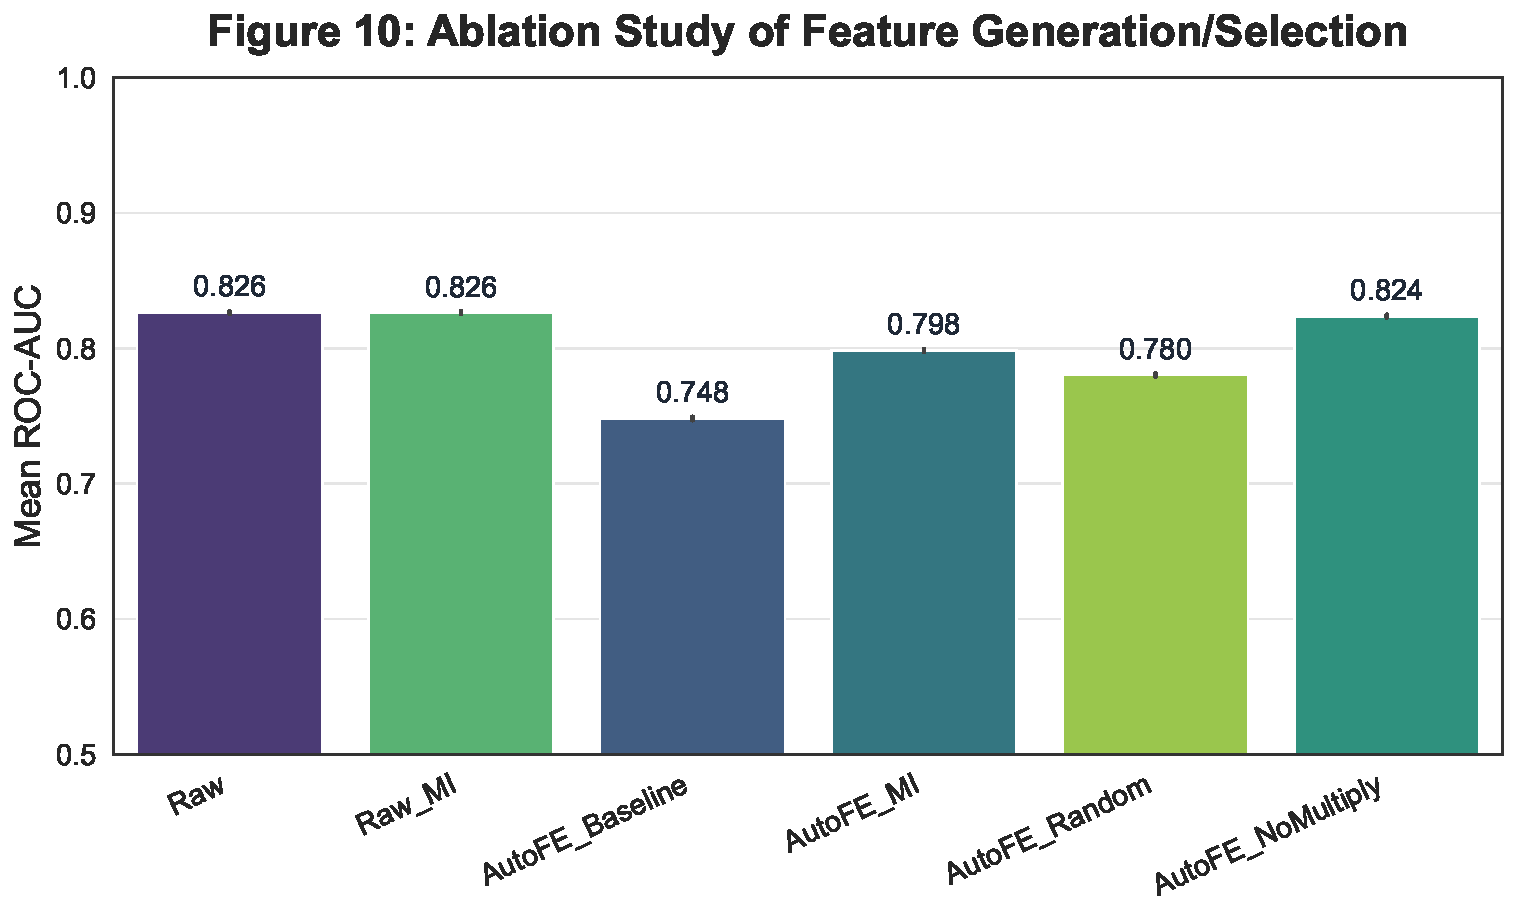
\includegraphics[width=0.80\textwidth]{Figure_10_Ablation_Study.pdf}
\caption{Ablation view of operator restrictions and selection variants.}
\label{fig:ablation}
\end{figure}

\subsection{Pairwise diagnostics}
Descriptive paired counts over the available task rows give 56,020 higher-Raw observations, 7,983 ties, and 10,887 lower-Raw observations for Raw versus AutoFE\_Baseline (74,890 paired records), and 31,954 higher-Raw observations, 20,914 ties, and 22,052 lower-Raw observations for Raw versus AutoFE\_NoMultiply.  The corresponding unpaired Cohen-style standardized differences in the recorded tables are $+0.5070$ and $+0.0189$.  These quantities are useful diagnostics, but repeated seeds, folds, conditions, and models create dependence; they are not independent data sets.  Figure~\ref{fig:nemenyi} therefore labels the regenerated matrix as a post-hoc diagnostic rather than a confirmatory critical-difference claim.

The data-set-by-pipeline heatmap in Figure~\ref{fig:heatmap} shows why a single pooled mean is insufficient.  The magnitude and even the local direction of the Raw--NoMultiply contrast vary across data sets, whereas the broad AutoFE\_Baseline is lower in nearly every row.  This heterogeneity motivates the data-set-balanced estimand and the paired uncertainty summaries reported above.

\begin{figure}[H]
\centering
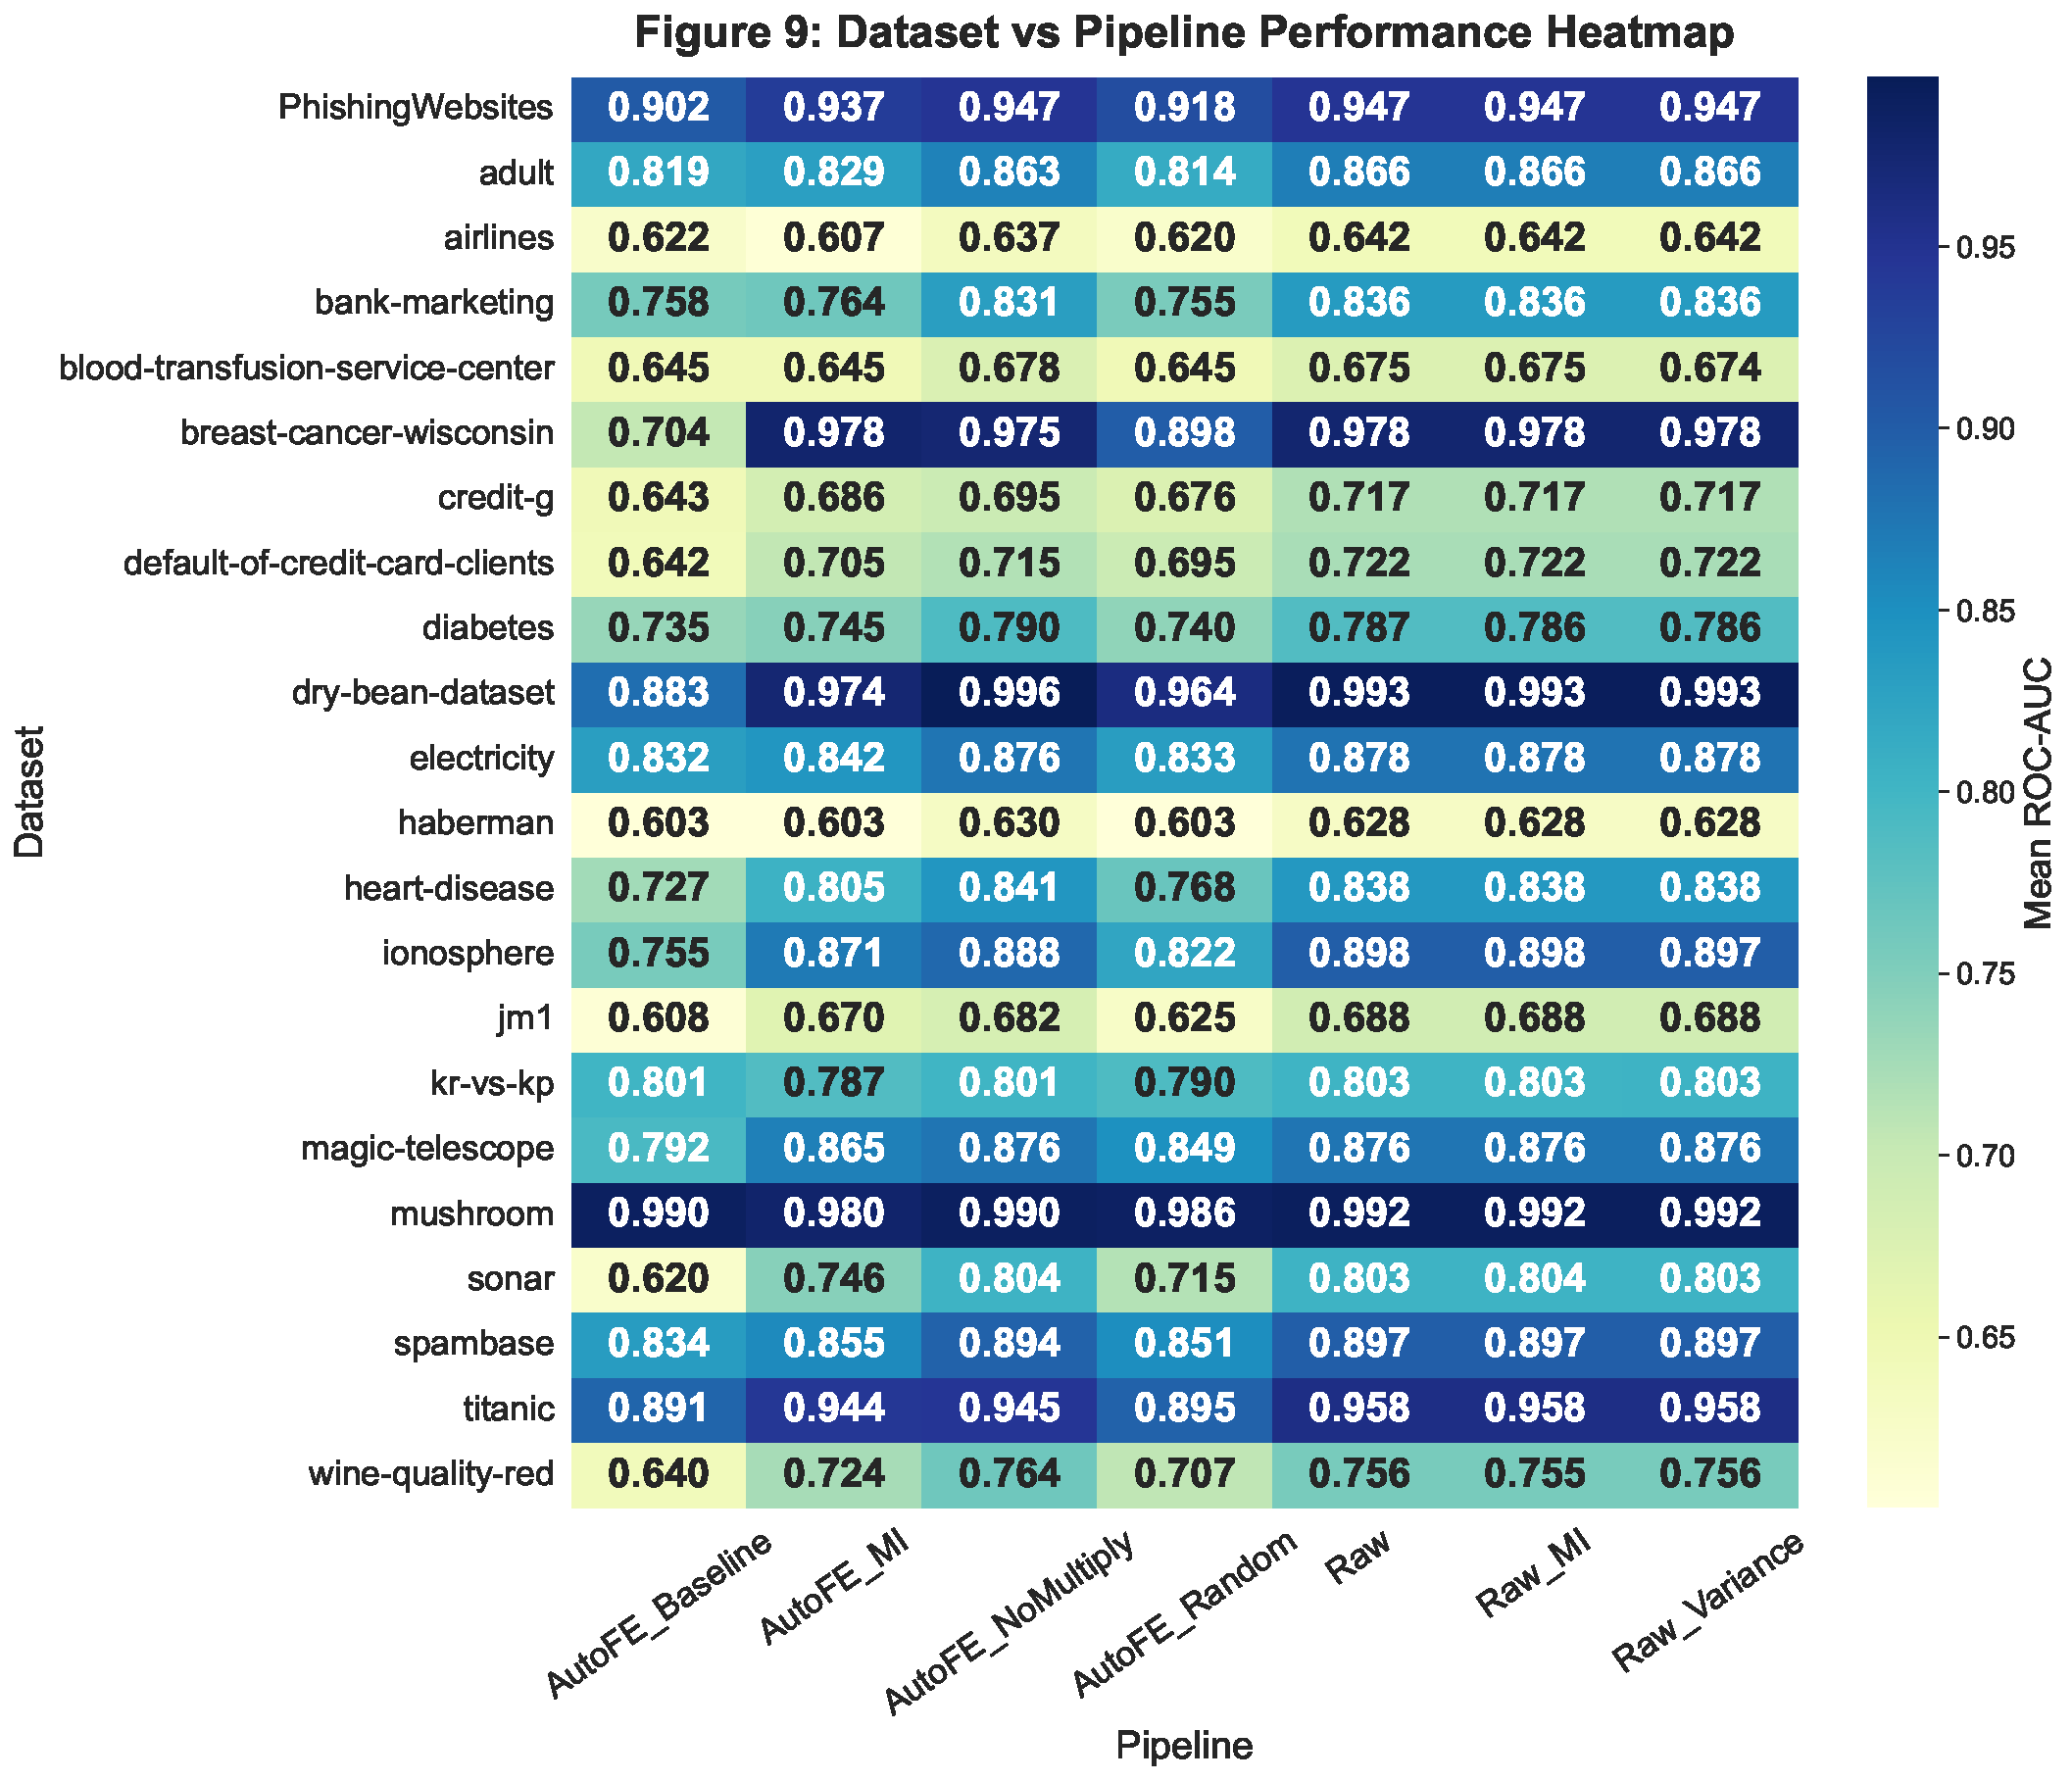
\includegraphics[width=0.96\linewidth]{Figure_9_Heatmap.pdf}
\caption{Data-set-by-pipeline mean ROC--AUC heatmap.  The panel exposes heterogeneity that is hidden by a single pooled benchmark mean.}
\label{fig:heatmap}
\end{figure}

\subsection{Statistical decision rule}
For a paired comparison at a fixed data set and task index, define $d_i=z_{i,p}-z_{i,q}$.  The signed-rank statistic is the sum of ranks of $|d_i|$ carrying positive signs, after removing zero differences.  For $k$ pipelines evaluated on $N$ matched data-set summaries, the Friedman statistic is
\begin{equation}
  \chi^2_F=\frac{12N}{k(k+1)}\left[\sum_{j=1}^{k}R_j^2-\frac{N k(k+1)^2}{4}\right],
\end{equation}
where $R_j$ is the sum of within-data-set ranks for pipeline $j$.  A Nemenyi comparison uses the mean-rank difference and standard error
\begin{equation}
  \operatorname{SE}=\sqrt{\frac{k(k+1)}{6N}},\qquad
  q_{pq}=\frac{|\overline R_p-\overline R_q|}{\operatorname{SE}}.
\end{equation}
These formulas clarify what a valid analysis would test.  The original pooled statistics instead use many correlated fold/seed/model rows and unpaired standardized differences.  We retain the figures for reproducibility, but we do not call their tiny pooled $p$-values a replication-level probability.  The recommended confirmatory analysis is a data-set-level paired bootstrap \citep{efron1979} or a mixed-effects model with data set as a random intercept, followed by Holm correction across the six primary pipeline contrasts \citep{holm1979}.  In that analysis, the estimand is the expected difference for a new data set, not the expected difference for a randomly selected checkpoint row.

\begin{figure}[H]
\centering
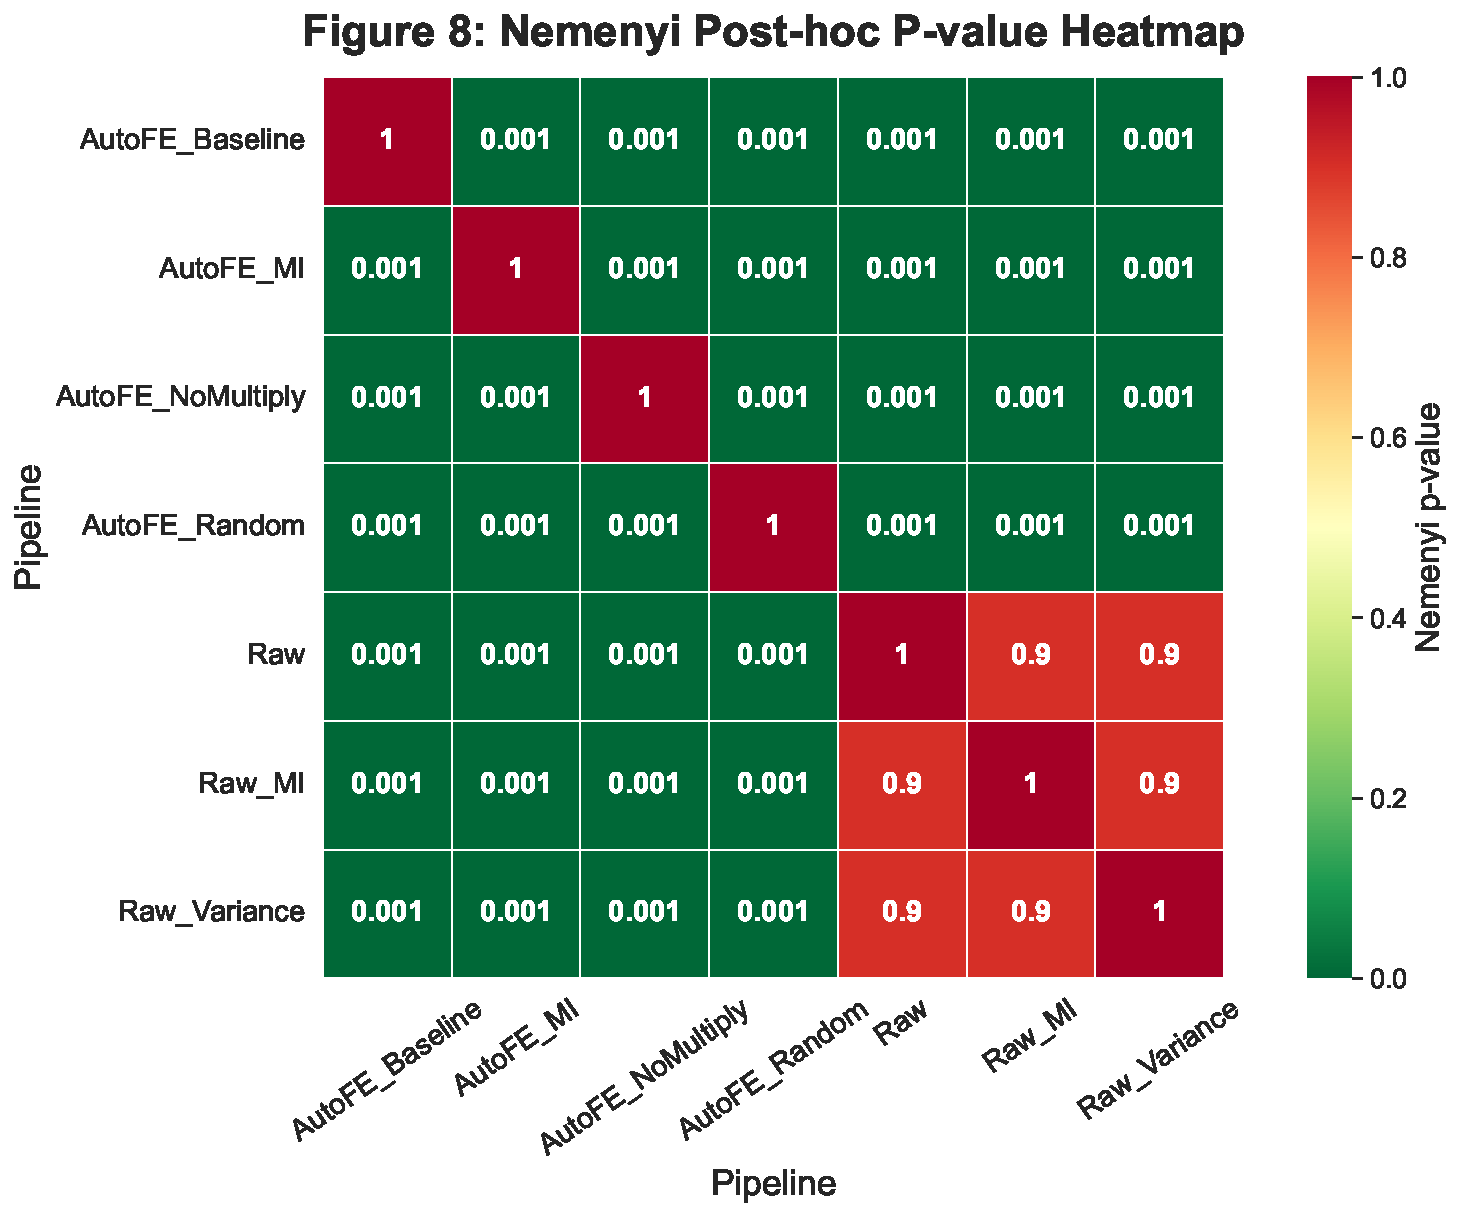
\includegraphics[width=0.80\textwidth]{Figure_8_CD_Diagram.pdf}
\caption{Directly regenerated Nemenyi-style pairwise $p$-value heatmap.  It is shown for diagnostic transparency; hierarchical reanalysis is required for confirmatory inference.}
\label{fig:nemenyi}
\end{figure}

\section{Discussion: implications for AutoML design}
\label{sec:discussion}

The central implication is architectural.  An AutoML system should not treat feature quantity as a proxy for feature quality.  The FSVA framework predicts that an operator library is useful only when its expected reduction in approximation bias exceeds the joint penalties from perturbation amplification, redundancy, conditioning, and search multiplicity.  Equation~\eqref{eq:fsva_master} turns that explanation into a compact design criterion: the representation is attractive only when its bias-reduction term offsets the other three terms.  The current results instantiate that regime boundary: unrestricted arithmetic synthesis is associated with a lower test AUC, a larger train--test gap, and a longer feature-generation tail, whereas the addition/subtraction restriction retains almost the raw-feature performance.

This observation suggests a robustness-aware AutoFE objective rather than a single clean-validation score.  Let $\mathcal{C}_{\mathrm{shift}}$ denote the specified training-corruption conditions, $T_p$ the median computational time, $M_p$ a memory summary, and $G_p$ an operator-sensitivity estimate such as the normalized Jacobian trace in Eq.~\eqref{eq:jacobian_amp}.  A deployable search objective can be written as
\begin{equation}
  \mathcal{J}(p)=\mu_{p,\mathrm{clean}}
  +\alpha\min_{c\in\mathcal{C}_{\mathrm{shift}}}
       \left(\mu_{p,c}-\mu_{p,\mathrm{clean}}\right)
  -\lambda_T\log(1+T_p)
  -\lambda_M\log(1+M_p)
  -\lambda_G G_p,
  \label{eq:automl_objective}
\end{equation}
where $\alpha,\lambda_T,\lambda_M,\lambda_G\ge0$ are selected on an inner validation layer.  Equation~\eqref{eq:automl_objective} changes the search question from ``which representation maximizes one score?'' to ``which representation provides stable predictive value per unit of computational and perturbation risk?''

\subsection{Feature quality rather than feature quantity}
To make the quality--cost claim operational, we define a descriptive Feature Utility Ratio (FUR) relative to a reference pipeline $r$.  Let $T_p$ be the median total time for pipeline $p$ across completed records, including feature generation, training, and inference.  For a small time floor $\tau_T>0$,
\begin{equation}
  \mathrm{FUR}(p\mid r)=
  \frac{\mu_p-\mu_r}{\max\{T_p-T_r,\tau_T\}},
  \qquad
  T_p=\operatorname{median}_{i\in\mathcal{I}}
  \left(t^{\mathrm{gen}}_{pi}+t^{\mathrm{train}}_{pi}+t^{\mathrm{infer}}_{pi}\right),
  \label{eq:fur}
\end{equation}
where $\mathcal{I}$ is the set of completed primary-scope records and $\mu_p$ is the data-set-balanced mean ROC--AUC.  FUR has units of AUC per additional second; a negative value means that the pipeline paid extra computation while losing predictive performance relative to $r$.  It is a within-benchmark diagnostic rather than a hardware-independent utility theorem, because both the timing denominator and the aggregation unit can change across implementations.

With Raw as $r$, the completed ledger gives median total times of 0.1481~s for Raw, 0.5663~s for AutoFE\_NoMultiply, 4.7450~s for AutoFE\_MI, 0.9831~s for AutoFE\_Random, and 1.0811~s for AutoFE\_Baseline.  Their corresponding FUR values are $-0.0062$, $-0.0061$, $-0.0549$, and $-0.0838$~AUC~s$^{-1}$, respectively.  Thus the broadest synthesis has the least favorable quality-adjusted cost: it adds the most computation while producing the largest negative AUC contrast.  Reporting this ratio alongside raw performance prevents a feature-generation system from being rewarded for expensive activity that does not survive held-out evaluation.

Three design principles follow.  First, candidate generation should be operator-aware: multiplication and division should be admitted when their empirical sensitivity and denominator stability are acceptable, not merely because they enlarge the library.  Second, candidate selection should report stability across folds, seeds, and corruption conditions, together with the effective-rank and condition-number diagnostics in Eqs.~\eqref{eq:coef_var}--\eqref{eq:effective_df}.  Third, the search budget should be explicit.  A feature with a small marginal AUC gain but a large increase in $\mathcal{J}$ is not an improvement for a production AutoML system, even if it wins a single clean validation split.

The implications extend to context-aware or LLM-assisted feature generation.  Semantic context can reduce the candidate library by proposing domain-plausible transformations \citep{muller2023}, but the generated code remains an operator map and is therefore subject to the same Jacobian, redundancy, and search-multiplicity analysis.  A robust AutoML system should log the provenance of every generated feature, its operator tree, its fold-wise selection frequency, its perturbation sensitivity, and its computational cost.  These records would allow FSVA to be tested directly rather than inferred from aggregate performance.

These results support a design recommendation: future AutoFE systems should jointly optimize feature quality, stability, and cost, with operator restrictions and robustness-aware objectives included in the search space.  The relevant regularization acts on the operator library, selection multiplicity, and perturbation sensitivity of the representation.  Future evaluations should therefore ask which generated features remain reliable when the data are imperfect.

\section{Reproducibility and computational specification}
\label{sec:reproducibility}

The executable protocol is organized around a YAML data-set list, a phase-one split/perturbation/preprocessing stage, and a phase-two model-evaluation stage.  Each completed task is checkpointed by the tuple $(d,s,f,c,p,m)$ in both JSONL and SQLite formats.  The configured environment pins NumPy 1.26.4, pandas 2.2.3, scikit-learn 1.5.2, SciPy 1.13.1, and Featuretools 1.31.0.  OpenML downloads are capped at 100,000 rows and sampled with seed 42 when necessary.  CPU and GPU estimator families can run concurrently; the runner records elapsed times but does not normalize for hardware, thermal state, or contention.

The paper assets are generated by \texttt{src/plotting\_q1.py} from the primary JSONL ledger and by \texttt{src/create\_workflow\_diagram.py}.  The latter writes a vector PDF and a 300-DPI PNG using only Matplotlib primitives.  Generated ledgers, caches, reports, and raster previews are kept outside version control, while the canonical PDF figures are bundled in \texttt{paper/figures/}.  For a reproducible rerun, the following provenance tuple should be recorded for every task or manifest:
\begin{equation}
\begin{aligned}
  \mathcal{P}=\{&\text{dataset identifier and version},\ \text{download checksum},\\
  &\text{code commit},\ \text{library lockfile},\ \text{hardware},\\
  &\text{random-state policy}\}.
\end{aligned}
\end{equation}
Without $\mathcal{P}$, a future run can reproduce the nominal grid but cannot establish bit-level identity with the current ledger.  This distinction is central to treating the current results as a reproducible benchmark snapshot rather than a final software release.

\section{Threats to validity and reproducibility}
\label{sec:limitations}

\paragraph{Incomplete data-set coverage.} The configured grid was not completed.  The primary analysis explicitly excludes the partial \texttt{kddcup99} and \texttt{covertype} blocks and the absent \texttt{aps\_failure} data set.  The stopping decision is part of the computational record, not a hidden negative result.  The missingness of long-running tasks can induce survivorship bias in pooled summaries.

\paragraph{Meaning of ``shift.''} Perturbations are applied to training data while the test partition remains clean.  Covariate and population conditions also receive the full data frame, including the numeric target, before partitioning.  The benchmark therefore supports statements about sensitivity to specified training-data corruption, not a clean estimate of deployment-time distribution shift.

\paragraph{Selection and leakage control.} The runner uses ordinary repeated five-fold tasks, not a complete nested model-selection protocol.  Although preprocessing and feature generation are intended to be fold-local, the global-data PCA/K-means representations used by the covariate/population splitters can expose target information through the partition geometry.  The reported performance should therefore be interpreted as benchmark performance under the implemented protocol, not as an unbiased estimate of a production model-selection pipeline.

\paragraph{Pipeline comparability.} All pipelines are capped at 20 preprocessed columns before model fitting, so Raw, Raw\_Variance, and Raw\_MI are near-duplicates.  AutoFE\_NoMultiply removes multiplication and division.  These design choices are informative ablations, but they are not a universal comparison of raw data with every possible AutoFE search space.

\paragraph{Randomness and checkpoints.} The perturbation seed uses Python’s salted \texttt{hash} function, which can change between interpreter processes.  Checkpoint keys do not encode data, code, or library versions, and worker exceptions are written to logs rather than emitted as failed result records.  Consequently, the 560,002 ledger entries are completed records, not a guaranteed accounting of every attempted task.

\paragraph{Target and metric semantics.} The implementation label-encodes target classes as integers but passes the original class labels to parts of the metric layer.  Binary ROC--AUC remains interpretable for the primary comparisons, whereas multiclass PR--AUC is often undefined and the multiclass Brier implementation is not valid without a consistent one-vs-rest encoding.  Distribution-distance fields compare transformed versions of the unchanged test partition and can therefore be zero even when the training partition was strongly corrupted.

\paragraph{Metrics and statistical units.} Non-standard JSON \texttt{NaN} values, unavailable multiclass PR--AUC, and invalid multiclass Brier label handling limit calibration claims.  Row-level tests also pseudoreplicate related folds, seeds, models, and conditions.  A stronger confirmatory analysis would rerun the experiment with stable seeds, explicit failure records, provenance, data-set-level aggregation, and hierarchical multiplicity-controlled inference.

\section{Conclusion}
\label{sec:conclusion}

The completed benchmark provides a bounded answer to the four questions.  Unrestricted arithmetic synthesis does not improve held-out ROC--AUC in the completed scope: the raw-feature mean exceeds AutoFE\_Baseline on all 22 data sets, with a mean gap of 0.0786 AUC.  Restricting the search to addition and subtraction removes almost all of that penalty: AutoFE\_NoMultiply differs from the raw-feature reference by only 0.0025 on average and is higher on eight data sets.  The broad variants also have larger train--test gaps, greater sensitivity to training missingness, and heavier feature-generation tails.  The evidence does not show that every AutoFE method is harmful.  It shows that a representation-search claim is incomplete unless it specifies the operator algebra, feature cap, aggregation unit, corruption semantics, failure accounting, and computational budget.  A second confirmatory run should address the stable-seed, provenance, failure-record, target-leakage, and hierarchical-inference issues in Section~\ref{sec:limitations}.  Future AutoFE systems should generate fewer, more stable, and theoretically justified features instead of treating feature count as evidence of progress.

\section*{CRediT authorship contribution statement}
Md. Shoaib Uddin Chanda: Conceptualization, Methodology, Software, Investigation, Data curation, Visualization, Writing, original draft, Writing, review and editing.  Mohammed Abdur Razzaq, Mohammed Abdul Razzak, and Ayesha Mahveen: Conceptualization, Software, Formal analysis, Investigation, Validation, Data curation, and Writing, review and editing, with equal contributions.  Their shared work included experiment execution, run logging, debugging, result verification, and manuscript development.

\section*{Declaration of competing interest}
The authors declare no known competing financial interests or personal relationships that could have appeared to influence the work reported in this paper.

\section*{Declaration of generative AI and AI-assisted technologies in the writing process}
During preparation of this manuscript, generative AI tools were used for language editing, document organization, code inspection, and figure-generation assistance.  The authors retained responsibility for the experimental design, source-data verification, numerical checks, interpretation, references, and final text, and reviewed all AI-assisted material before inclusion.  No generative AI system is listed as an author.

\section*{Ethics statement}
The study analyzes public, tabular benchmark data accessed through OpenML and does not collect new personal data or intervene with human participants.  Dataset use remains subject to the licensing and provenance information associated with the individual OpenML records.

\section*{Data availability}
The benchmark uses public OpenML data sources \citep{vanschoren2013}.  The source code, configuration, manuscript source, references, and canonical PDF figures are available at \url{https://github.com/mdshoaibuddinchanda/AutoFE-ShiftBench}.  Generated ledgers, caches, reports, and checkpoint databases are intentionally excluded from version control because of their size and reproducible origin; the local analysis archive retains the completed records used in this manuscript.

\section*{Funding}
This research received no external funding.

\bibliographystyle{elsarticle-harv}
\bibliography{references}

\end{document}
